\documentclass{report}
\usepackage[margin=2cm, bottom=1.5cm]{geometry}
\usepackage{type1cm}
\usepackage{amssymb}
\usepackage[fleqn]{amsmath}
\usepackage{tikz}
\usepackage{multicol}
\usepackage{makecell}
\usepackage{tabularx}
\usepackage[shortlabels]{enumitem}
\setlength{\columnsep}{1pt}
\setlist[enumerate]{nosep}

\makeatletter
\newenvironment{myalign*}{\ifvmode\else\hfil\null\linebreak\fi
  \hspace*{-\leftmargin}\minipage\textwidth
  \setlength{\abovedisplayskip}{0pt}%
  \setlength{\abovedisplayshortskip}{\abovedisplayskip}%
  \start@align\@ne\st@rredtrue\m@ne}%
{\endalign\endminipage\linebreak}

\usepackage{xeCJK}
\setCJKmainfont{Noto Sans TC}

\begin{document}
\title{%
  \fontsize{40}{60}\selectfont
  SCAF  \\ % 
  \vspace*{2cm}%
  \fontsize{24}{30}\selectfont
  需求規格文件
}

\author{
  \fontsize{18}{28}\selectfont
  \begin{tabularx}{0.9\textwidth}{
    |p{\dimexpr.25\linewidth-6\tabcolsep-2\arrayrulewidth}%
    |p{\dimexpr.75\linewidth-6\tabcolsep-2\arrayrulewidth}|%
  }
    \hline
    \centering 專案名稱 & SCAF 開發輔助工具 \\
    \hline
    \centering 撰寫日期 & 2022 / 10 / 19 \\
    \hline
    \centering 發展者 & 簡蔚驊 \! 鄧暐宣 \! 余威霆 \! 林佳何 \! 唐劭賢 \\
    \hline
  \end{tabularx}
}
\date{}
\usetikzlibrary{automata, positioning, arrows}
\maketitle
\tikzset{every state, accepting/.style={double distance=2pt}}

\fontsize{12}{18}\selectfont

\section*{版次變更記錄}
\begin{tabularx}{\textwidth}{ 
  |p{\dimexpr.2\linewidth-2\tabcolsep-1.33333\arrayrulewidth}%
  |p{\dimexpr.6\linewidth-2\tabcolsep-1.33333\arrayrulewidth}%
  |p{\dimexpr.2\linewidth-2\tabcolsep-1.33333\arrayrulewidth}|%
}
  \hline
  版次 & 變更項目 & 變更日期 \\
  \hline
  1.0 & 初版 & 2022 / 10 / 19 \\
  \hline
  1.1 & 
  \makecell[l]{
    1. 補上操作概念 \\
    2. 補上使用者地圖 \\
  }
  & 2022 / 11 / 03 \\
  \hline
  1.2 & 
  \makecell[l]{
    1. 登入功能刪除第三方登入 \\
    2. 專案初始化功能刪除前後端基本的文件,添加外部的\\
    插件 \\
    3. 專案初始化功能新增增加README \\
    4. 新增建立repository連結功能 \\
    5. 刪除整合其他工具功能 \\
    6. 刪除自動化測試功能 \\
    7. 刪除自動化部署功能 \\
    8. 刪除產生規範文件功能 \\
    9. 刪除版本控管功能 \\ 
    10. 新增專案管理功能 \\
    11. 新增專案修改功能 \\
    12. 新增Google日曆授權功能 \\
  }
  & 2022 / 12 / 17 \\
  \hline
  1.3 & 
  \makecell[l]{
    1. 補上註冊CLI操作概念 \\
    2. 補上登入CLI操作概念\\
    3. 補上忘記密碼CLI操作概念\\
    4. 補上初始化專案CLI操作概念\\
    5. 補上repo CLI操作概念\\
    6. 補上看板CLI操作概念\\
    7. 補上文件編輯CLI操作概念\\
    8. 補上專案設定CLI操作概念\\
    9. 補上專案管理CLI操作概念 \\
    10. 補上專案刪除CLI操作概念 \\
    11. 補上連結QA CLI操作概念 \\
  }
  & 2022 / 1 / 12 \\
  \hline
\end{tabularx}



\section*{0. 接受準則(Acceptance Criteria of this document)}
\begin{itemize}
  \item Clearly and properly stated (需求需清楚且適當的陳述)
  \item Complete (需求需完整)
  \item Consistent with each other (需求之間需維持一致性)
  \item Uniquely identified (每項需求有明確之識別)
  \item Appropriate to implement (需求需可被實作)
  \item Verifiable (需求需可被驗證)
\end{itemize}

\section*{1. 系統概述(System Description)}
目標: 以簡化的方式呈現 SCAF (Software Co-working Assistance Framework)的功能,
並且提供使用者一個簡單的操作介面,讓使用者能夠輕鬆的使用 SCAF 的功能。\\
特色: 簡單、易用、快速。\\
實作方案:
  \begin{itemize}
    \item 使用 Adobe XD (Adobe Experience Design)設計 UI 介面
    \item 使用 Vue 技術實現前端頁面
    \item 使用 Go 設計 CLI 工具
    \item 使用 Go 設計後端 API
  \end{itemize}
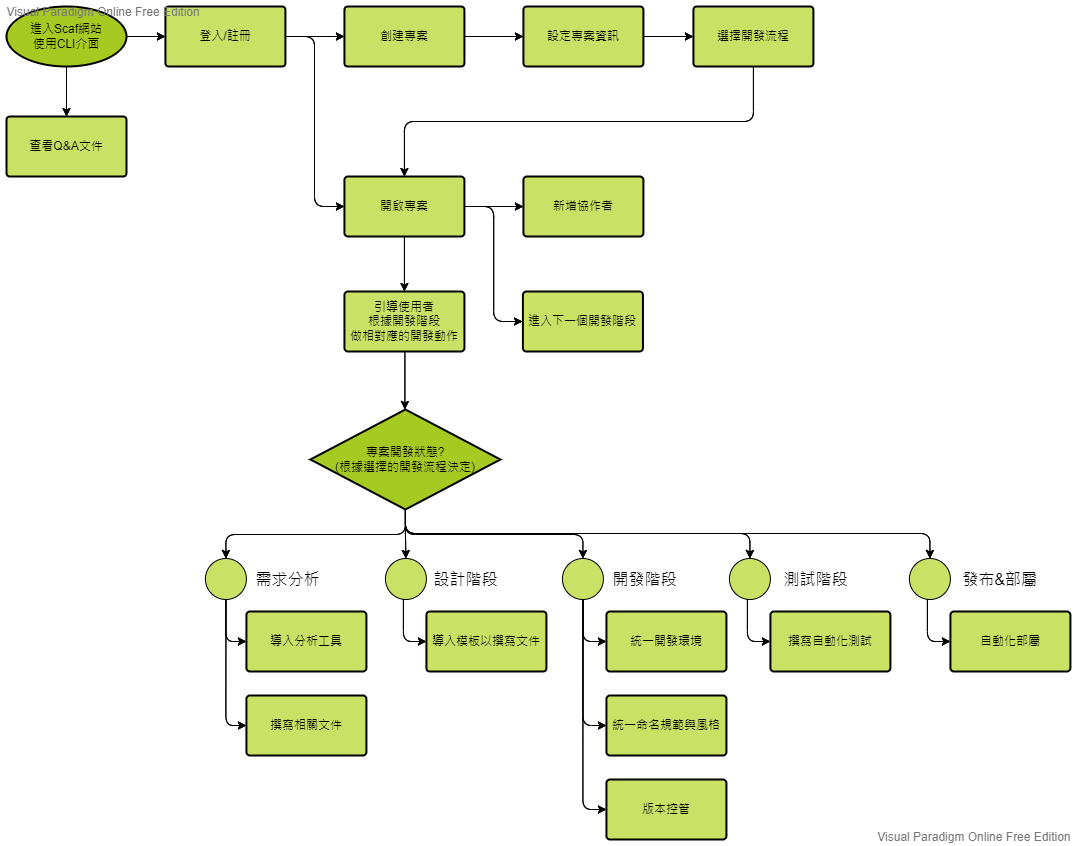
\includegraphics[width=\textwidth]{assets/system.png}

\section*{2. 使用者故事地圖(User Story Map)}

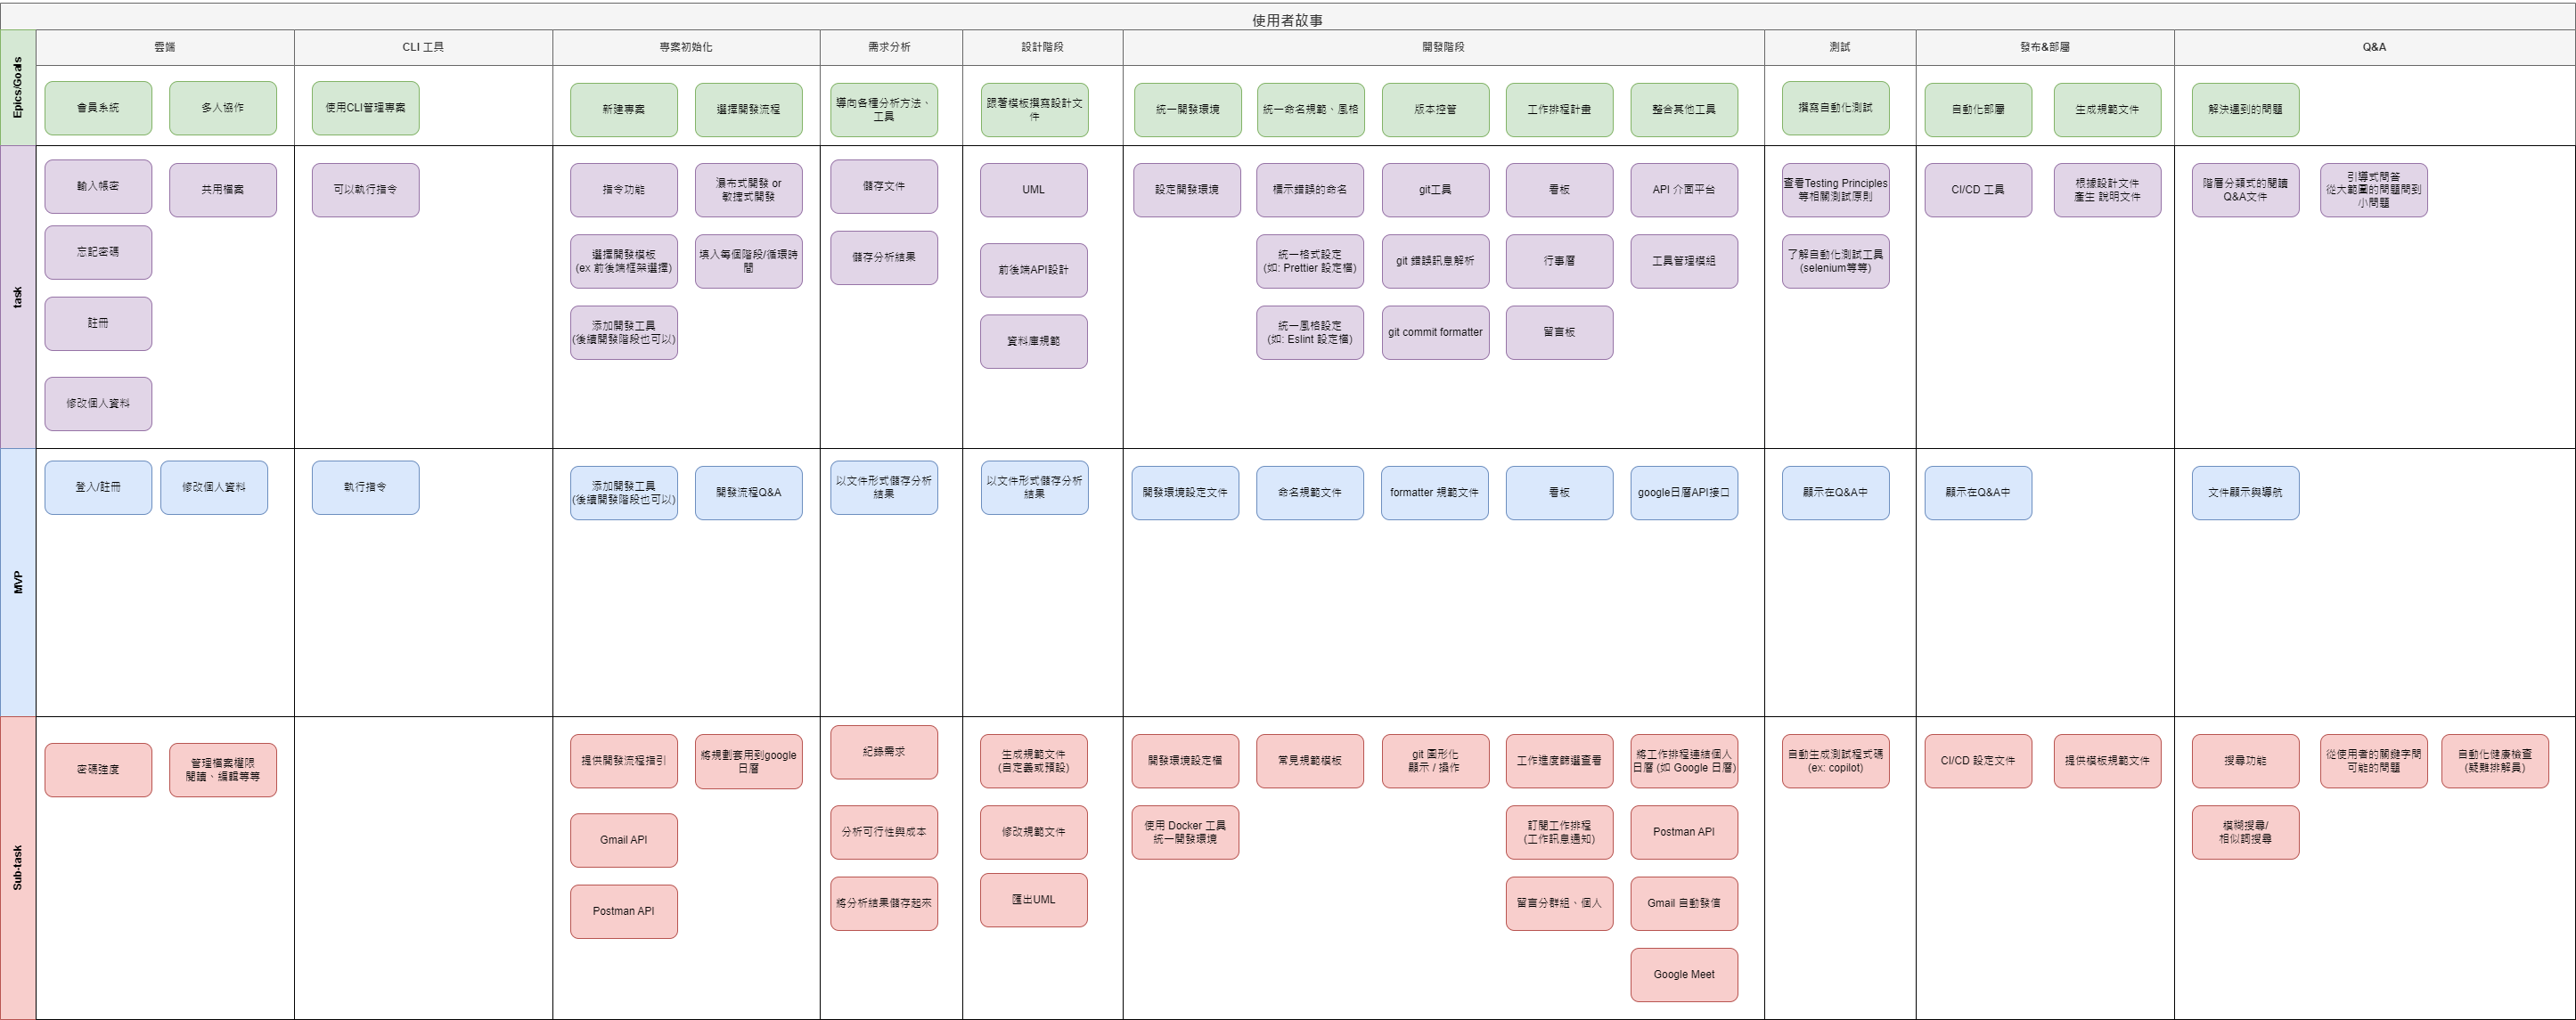
\includegraphics[width=\textwidth]{assets/User_Story_Map.png}

% \subsection*{}
% \fontsize{12}{20}\selectfont
% \begin{tabularx}{\textwidth}{|X|}
%   \hline
%   代號:\\ \hline
%   故事: \\ \hline
%   註記: \\ \hline
%   測試方案: \\ \hline
% \end{tabularx}

\subsection*{}
\fontsize{12}{20}\selectfont
\begin{tabularx}{\textwidth}{|X|}
  \hline
  代號:SCAF-US-01 登入\\ \hline
  故事:作為一個使用者我可以輸入已註冊的帳號登入這個系統。 \\ \hline
  註記:
  \begin{enumerate}
    \item 登入要輸入電子郵件和密碼
    \item 登入失敗會出現錯誤訊息
    \item 使用者可以使用第三方登入 
  \end{enumerate} \\ \hline
  測試方案:
  \begin{enumerate}
    \item 輸入未註冊的電子郵件與密碼,確認是否失敗與顯示錯誤訊息
    \item 辦完帳號以後,輸入電子郵件以及密碼看是否能登入
    \item 使用第三方登入,確認是否能夠連動
  \end{enumerate} \\ \hline
\end{tabularx}

\subsection*{}
\fontsize{12}{20}\selectfont
\begin{tabularx}{\textwidth}{|X|}
  \hline
  代號:SCAF-US-02 註冊 \\ \hline
  故事:作為一個使用者我可以註冊新帳戶或連動第三方應用程式,讓我可以登入這個系統。 \\ \hline
  註記:
  \begin{enumerate}
    \item 註冊時需輸入電子郵件、用戶名、密碼
    \item 註冊電子郵件為無效的電子郵件,出現錯誤訊息
  \end{enumerate} \\ \hline
  測試方案:
  \begin{enumerate}
    \item 若註冊時輸入無效的 email,確認是否有錯誤訊息
  \end{enumerate} \\ \hline
\end{tabularx}

\subsection*{}
\fontsize{12}{20}\selectfont
\begin{tabularx}{\textwidth}{|X|}
  \hline
  代號:SCAF-US-03 修改個人資料 \\
  \hline
  故事:作為一個使用者,我要能夠修改自己的個人資料,像是使用者名稱太中二
想修改、密碼取得太簡單想改困難一點、想取消第三方的應用程式連動。 \\
  \hline
  註記:
  \begin{enumerate}
    \item 使用者可以修改名稱,並自動登出
    \item 使用者可以修改密碼,並自動登出
    \item 使用者可以新增或取消第三方應用程式連動,並自動登出
    \item 系統提醒使用者確認變更
    \item 修改名稱或密碼時,未輸入字元送出,出現錯誤訊息
  \end{enumerate} \\
  \hline
  測試方案:
  \begin{enumerate}
    \item 修改名稱或密碼時,未輸入字元送出,確認是否有錯誤訊息
    \item 修改使用名稱後,重新登入,進入系統看是否為新名稱
    \item 新增或取消第三方應用程式連動後,重新登入,查看是否可以正常登入
    \item 修改密碼後,再用新密碼登入,確認是否能成功登入
    \item 修改名稱後,確認是否自動登出
    \item 修改密碼後,確認是否自動登出
    \item 新增或取消第三方應用程式連動後,確認是否自動登出
  \end{enumerate} \\
  \hline
\end{tabularx}

\subsection*{}
\fontsize{12}{20}\selectfont
\begin{tabularx}{\textwidth}{|X|}
  \hline
  代號:SCAF-US-04 執行命令 \\
  \hline
  故事:作為一個使用者,我能夠進入CLI介面並在此輸入我想要的指令,像是使用init來初始化專案。 \\
  \hline
  註記:
  \begin{enumerate}
    \item 指令有固定的格式規範
    \item 有help指令可以查看指令的說明
    \item 所有網站的功能都可以透過指令來執行
    \item 輸入指令時,輸入錯誤的指令,會出現錯誤訊息
  \end{enumerate} \\
  \hline
  測試方案:
  \begin{enumerate}
    \item 輸入指令時,輸入錯誤的指令,確認是否有錯誤訊息
    \item 輸入指令時,輸入正確的指令,確認是否有正確執行
    \item 輸入指令時,輸入 help,確認是否有列出所有指令
    \item 輸入指令時,輸入 help 指令,確認是否有列出該指令的說明
  \end{enumerate} \\
  \hline
\end{tabularx}

\subsection*{}
\fontsize{12}{20}\selectfont
\begin{tabularx}{\textwidth}{|X|}
  \hline
  代號:SCAF-US-05 添加開發工具 \\
  \hline
  故事:作為一個使用者,我能夠在專案開始時(或是後續開發階段), 選擇系統的選項,並查看系統所推薦的開發工具,或者自行添加開發工具。 \\
  \hline
  註記:
  \begin{enumerate}
    \item 系統會有幾個固定選項,使用者可以選擇其中一個
    \item 若不滿意系統推薦的選項,使用者可以自行添加開發工具
    \item 後續的開發階段,使用者可以選擇更換開發工具
  \end{enumerate} \\
  \hline
  測試方案:
  \begin{enumerate}
    \item 在專案開始時,使用者可以選擇其中一個固定選項
    \item 添加完開發工具後,進入專案,確認是否有正確添加
    \item 移除開發工具後,進入專案,確認是否有正確移除
  \end{enumerate} \\
  \hline
\end{tabularx}

\subsection*{}
\fontsize{12}{20}\selectfont
\begin{tabularx}{\textwidth}{|X|}
  \hline
  代號:SCAF-US-06 開發、測試、發布\&部屬 Q\&A \\
  \hline
  故事:作為一個使用者,當我對於開發、測試、發布\&部屬流程有所疑惑時,可以打開開發流程Q\&A文件,查看自己的疑惑是否在常見問題中。 \\
  \hline
  註記:
  \begin{enumerate}
    \item 文件會條列出流程階段的常見問題
    \item 提供關鍵字搜尋功能
    \item 文件會條列出相關資料
    \item 文件會條列出各個領域中常見的問題
    \item 文件會條列出相關工具的資料
    \item 提供關鍵字搜尋功能 (搜尋google還是在文件內搜尋?)
  \end{enumerate} \\
  \hline
  測試方案:
  \begin{enumerate}
    \item 點開文件,確認是否有列出常見問題
    \item 點開文件,確認是否有列出相關資料
    \item 輸入不存在的關鍵字,確認是否有顯示沒有找到相關問題
    \item 點開某個Q\&A確認,內容是否與點擊的相同
  \end{enumerate} \\
  \hline
\end{tabularx}

\subsection*{}
\fontsize{12}{20}\selectfont
\begin{tabularx}{\textwidth}{|X|}
  \hline
  代號:SCAF-US-07 需求分析、設計階段、開發環境設定、命名規範、git commit format規範 以文件形式儲存分析結果 \\
  \hline
  故事:作為一個使用者,當我在撰寫需求文件時,我能夠將我的文件處存在此軟體中,並在我需要時叫出它做修改。 \\
  \hline
  註記:
  \begin{enumerate}
    \item 將使用hackmd撰寫的文件,儲存在此軟體中
    \item 更改文件後,可以讓更改者決定是否發文件通知所有人
    \item 規範文件會有一個獨立的頁面
  \end{enumerate} \\
  \hline
  測試方案:
  \begin{enumerate}
    \item 點開文件,確認是否內容相同
    \item 新增一個文件
    \item 編輯文件
    \item 刪除文件
    \item 更改文件後,選擇發送通知,確認每一個人都有收到通知
  \end{enumerate} \\
  \hline
\end{tabularx}

\subsection*{}
\fontsize{12}{20}\selectfont
\begin{tabularx}{\textwidth}{|X|}
  \hline
  代號:SCAF-US08 看板 \\
  \hline
  故事:作為一個使用者,我可以利用看板功能來紀錄與查看專案各個任務的開發進度,使團隊的協作與交付流程更加
  順暢。 \\
  \hline
  註記:
  \begin{enumerate}
    \item 任務可設定標籤、進度、成員、描述、時間排程
    \item 將任務放入看板中並依照任務的狀態分類,如:待處理、進行中、已完成
    \item 可對任務進行篩選查看
    \item 會發送訊息通知所有人,當有人將任務拖曳至看板中或任務狀態改變時
    \item 不同標籤的任務會以顏色區分
    \item 看板功能會有一個獨立的頁面
  \end{enumerate} \\
  \hline
  測試方案:
  \begin{enumerate}
    \item 新增一個任務至看板中,確認是否有顯示與發送通知
    \item 變更任務狀態,確認是否有顯示與發送通知
    \item 刪除一個任務,確認是否有顯示與發送通知
    \item 新增兩個不同標籤的任務,確認顏色是否相異
    \item 新增兩個相同標籤的任務,確認顏色是否相同
  \end{enumerate} \\
  \hline
\end{tabularx}

\subsection*{}
\fontsize{12}{20}\selectfont
\begin{tabularx}{\textwidth}{|X|}
  \hline
  代號:SCAF-US-09 google日曆API接口 \\
  \hline
  故事:作為一個使用者,我可以將看板任務的時間排程,同步到google日曆中,以便查看與管理時間。 \\
  \hline
  註記:
  \begin{enumerate}
    \item 可點擊授權按鈕,驗證完成後,將看板中所負責的任務同步到google日曆中
    \item 新增或變更任務時間排程後,會自動寄信至信箱中提醒負責人,並同步到負責人的google日曆中
    \item google日曆API接口功能會有一個獨立的頁面
    \item 輸入不合法的電子郵件,會出現錯誤訊息
  \end{enumerate} \\
  \hline
  測試方案:
  \begin{enumerate}
    \item 點擊授權按鈕,確認是否有成功授權
    \item 驗證過後,確認是否有將所負責的任務同步到google日曆中
    \item 新增任務,確認是否同步到google日曆中
    \item 變更任務時間排程,確認是否有同步到google日曆中
    \item 刪除任務,確認是否有同步到google日曆中
  \end{enumerate} \\
  \hline
\end{tabularx}

\subsection*{}
\fontsize{12}{20}\selectfont
\begin{tabularx}{\textwidth}{|X|}
  \hline
  代號:SCAF-US-10 Q\&A 文件顯示與導航 \\
  \hline
  故事:作為一個使用者,當我在Q\&A文件中,可以點選連結,導航到不同項目的Q\&A文件中,或是透過搜尋功能,找
  到相關的資料。 \\
  \hline
  註記:
  \begin{enumerate}
    \item 目錄中的連結可以導航到不同項目的Q\&A文件中
    \item 提供關鍵字搜尋功能
    % \item 提供模糊搜尋功能
    \item Q\&A文件是階層式的架構
  \end{enumerate} \\
  \hline
  測試方案:
  \begin{enumerate}
    \item 點開Q\&A文件,確認是否有列出目錄
    \item 點開目錄中的連結,確認是否有導航到不同項目的Q\&A文件中
    % \item 輸入空白的關鍵字,確認是否有顯示請輸入關鍵字
    \item 未輸入關鍵字就點擊搜尋,要顯示「請輸入關鍵字」
    \item 關鍵字搜尋輸入存在的關鍵字,確認是否有顯示相關資料
    \item 關鍵字搜尋輸入不存在的關鍵字,確認是否有顯示沒有找到相關資料
    % \item 模糊搜尋輸入關鍵字,確認是否有顯示相似的相關問題
  \end{enumerate} \\
  \hline
\end{tabularx}


\subsection*{3. 操作概念(Operation
 Concept)}

兩張圖的操作概念,第一張為網站的操作,第二張為CLI工具的操作

\begin{enumerate}[label=(\Alph*)]
  \item 會員註冊: 小林進入了這個 SCAF 平台,輸入名稱、信箱、密碼,註冊了一個帳號。 \\
  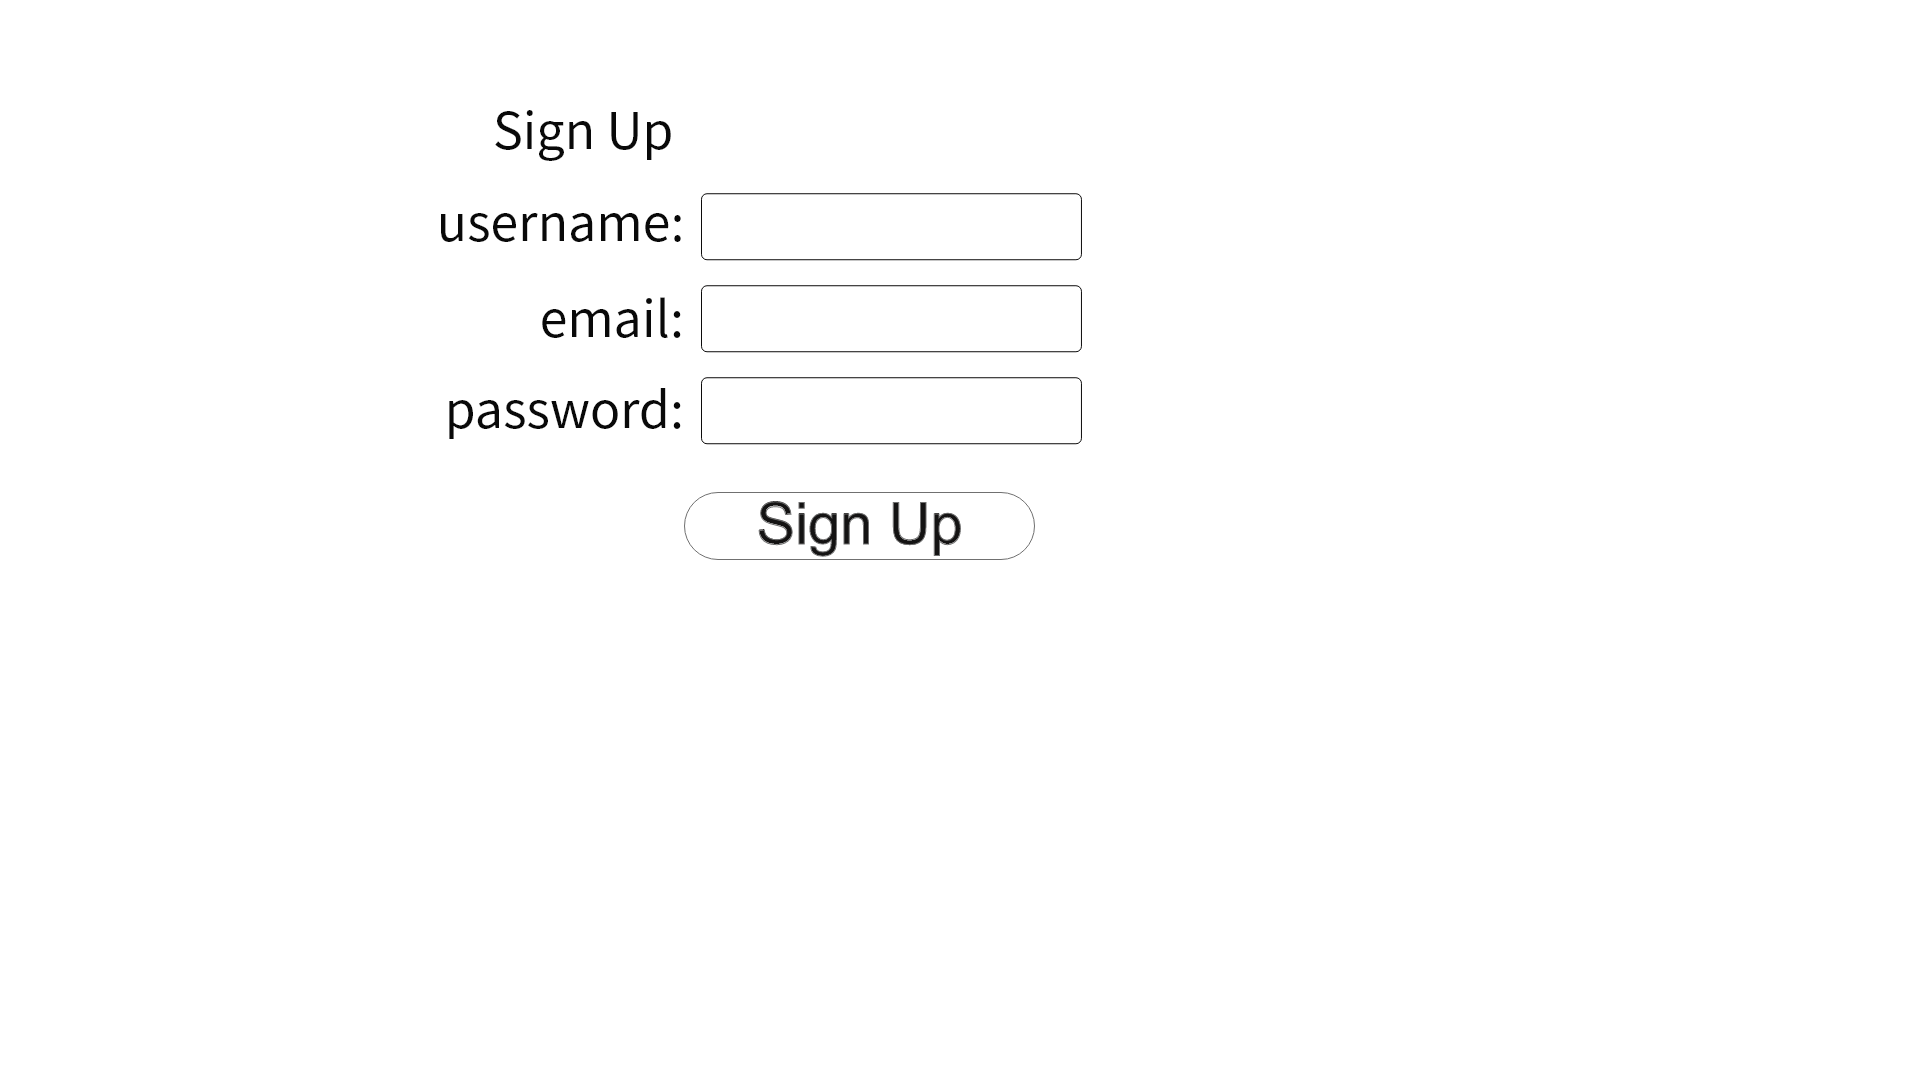
\includegraphics[width=\textwidth]{assets/wireframe/sign_up.png}
  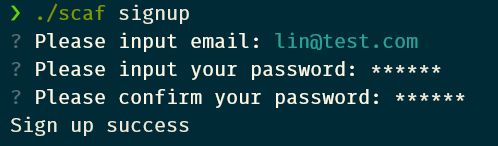
\includegraphics[width=\textwidth]{assets/wireframe/sign_up_CLI.png}
  \item 會員登入: 小林辦好帳號後,馬上試著登入平台來開始自己的軟體開發流程。 \\
  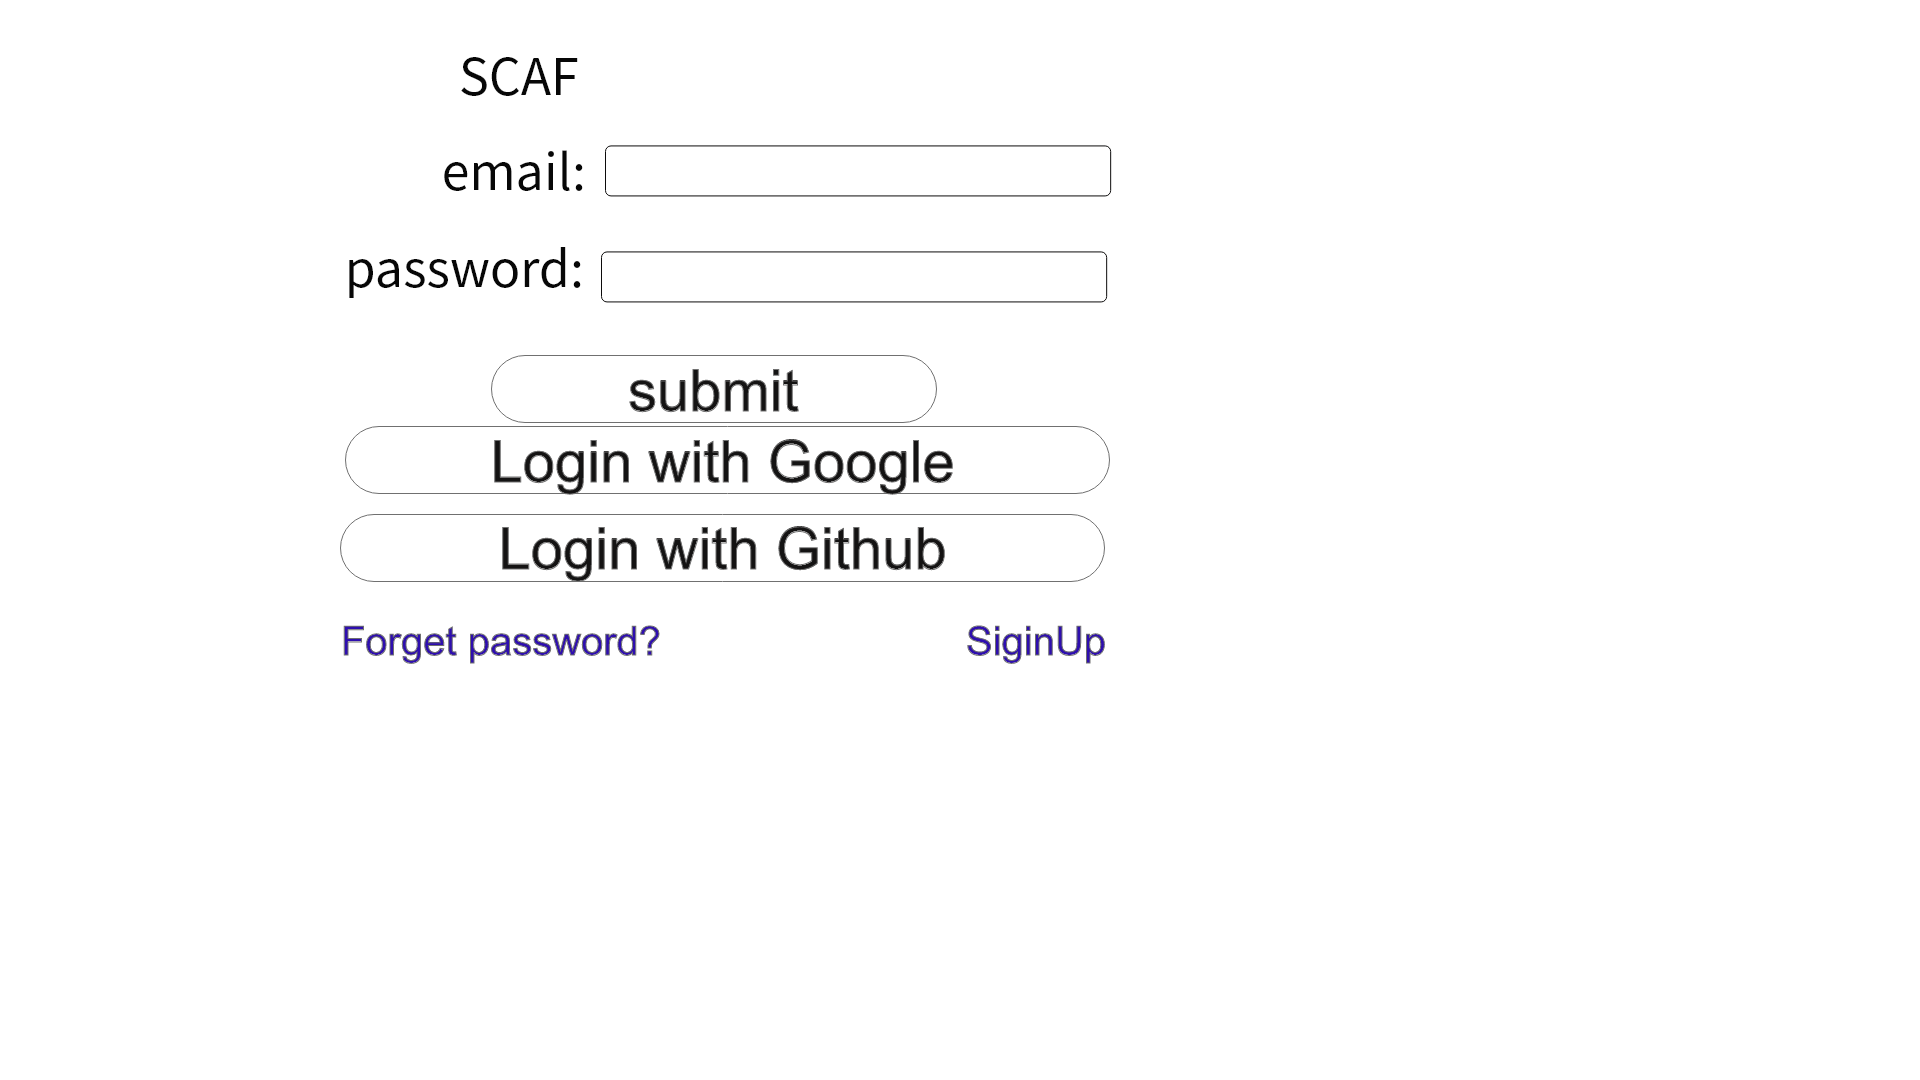
\includegraphics[width=\textwidth]{assets/wireframe/Login.png}
  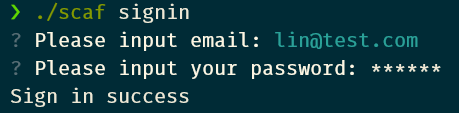
\includegraphics[width=\textwidth]{assets/wireframe/Login_CLI.png}
  \item 忘記密碼: 登入時卻發現,輸入好多次密碼都是錯的,只好重設密碼,輸入信箱之後,查看了自己的信箱,並點擊 Link 去重新設定密碼。\\
  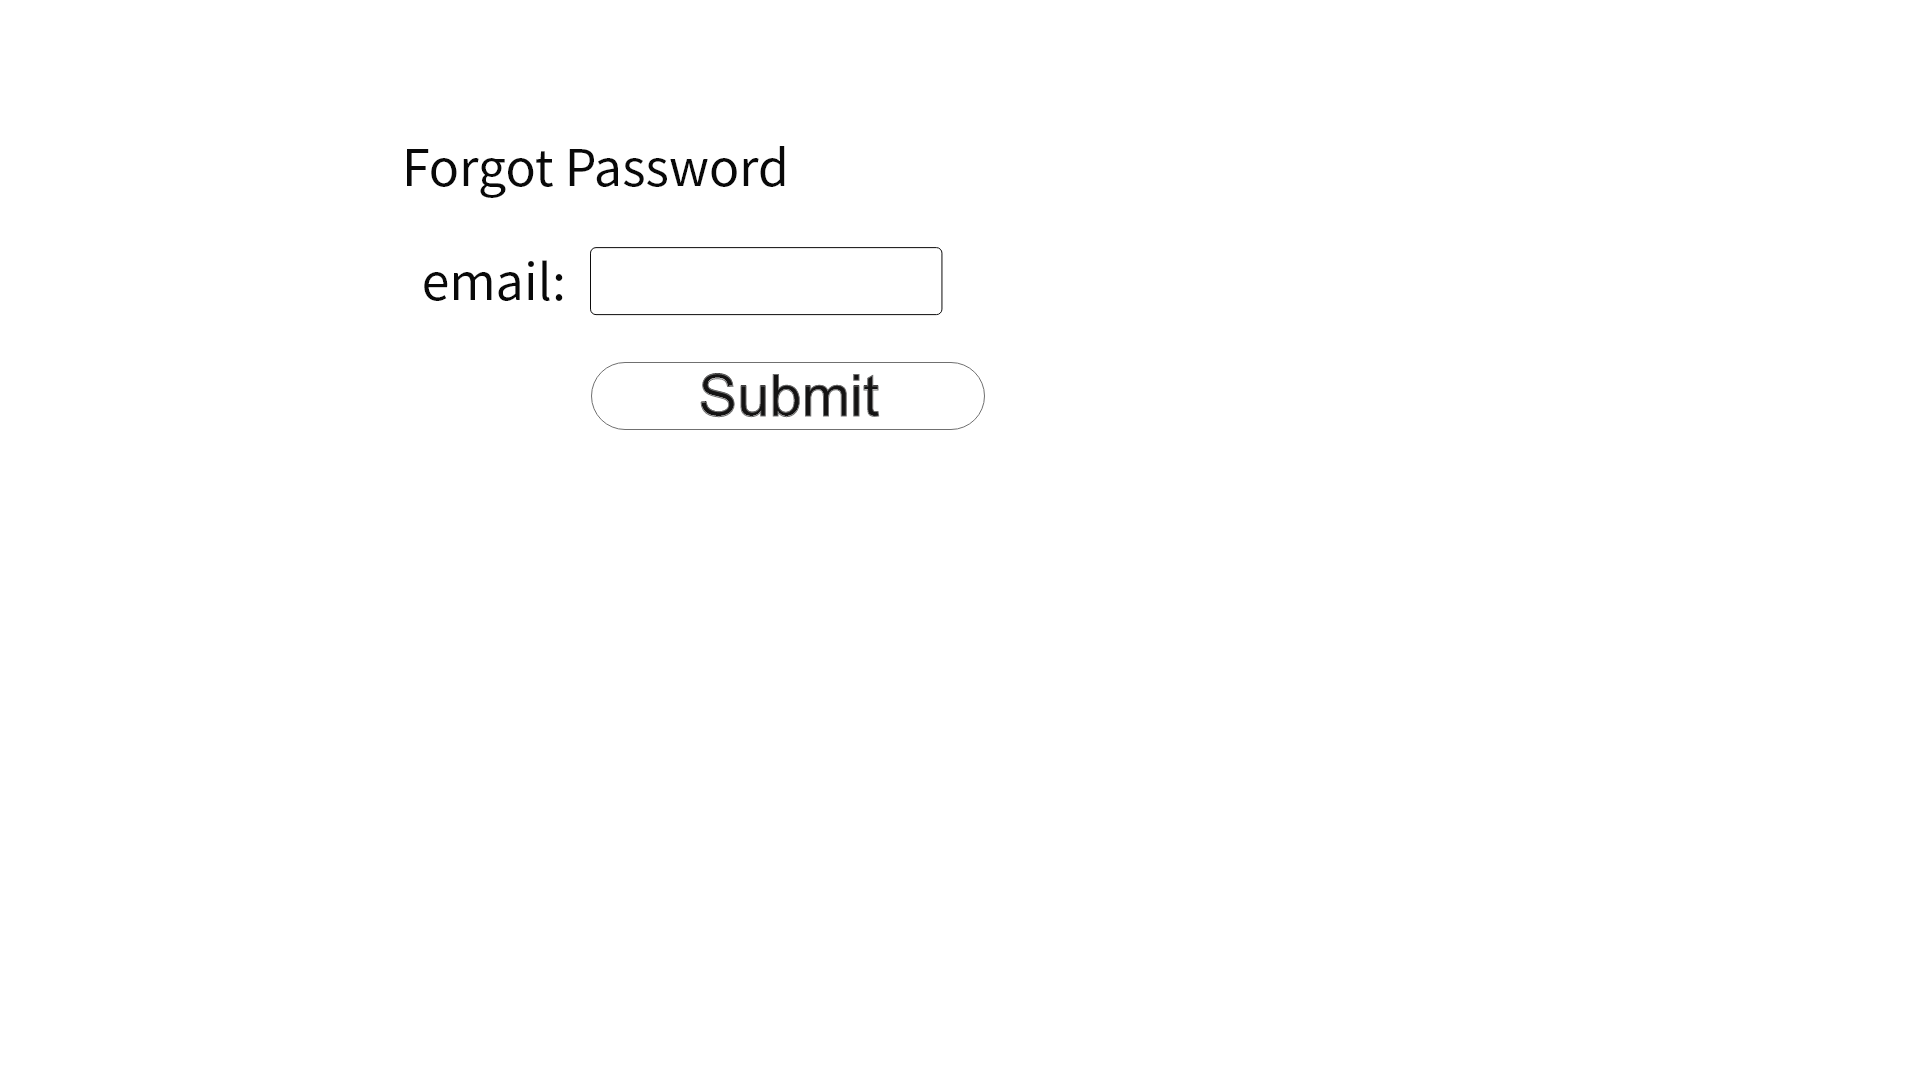
\includegraphics[width=\textwidth]{assets/wireframe/forgot_password.png}
  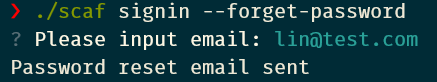
\includegraphics[width=\textwidth]{assets/wireframe/forgot_password_CLI.png}
  \item 新建專案: 小林進入系統之後立刻想要開始第一個專案,於是按下了+號鍵。\\
  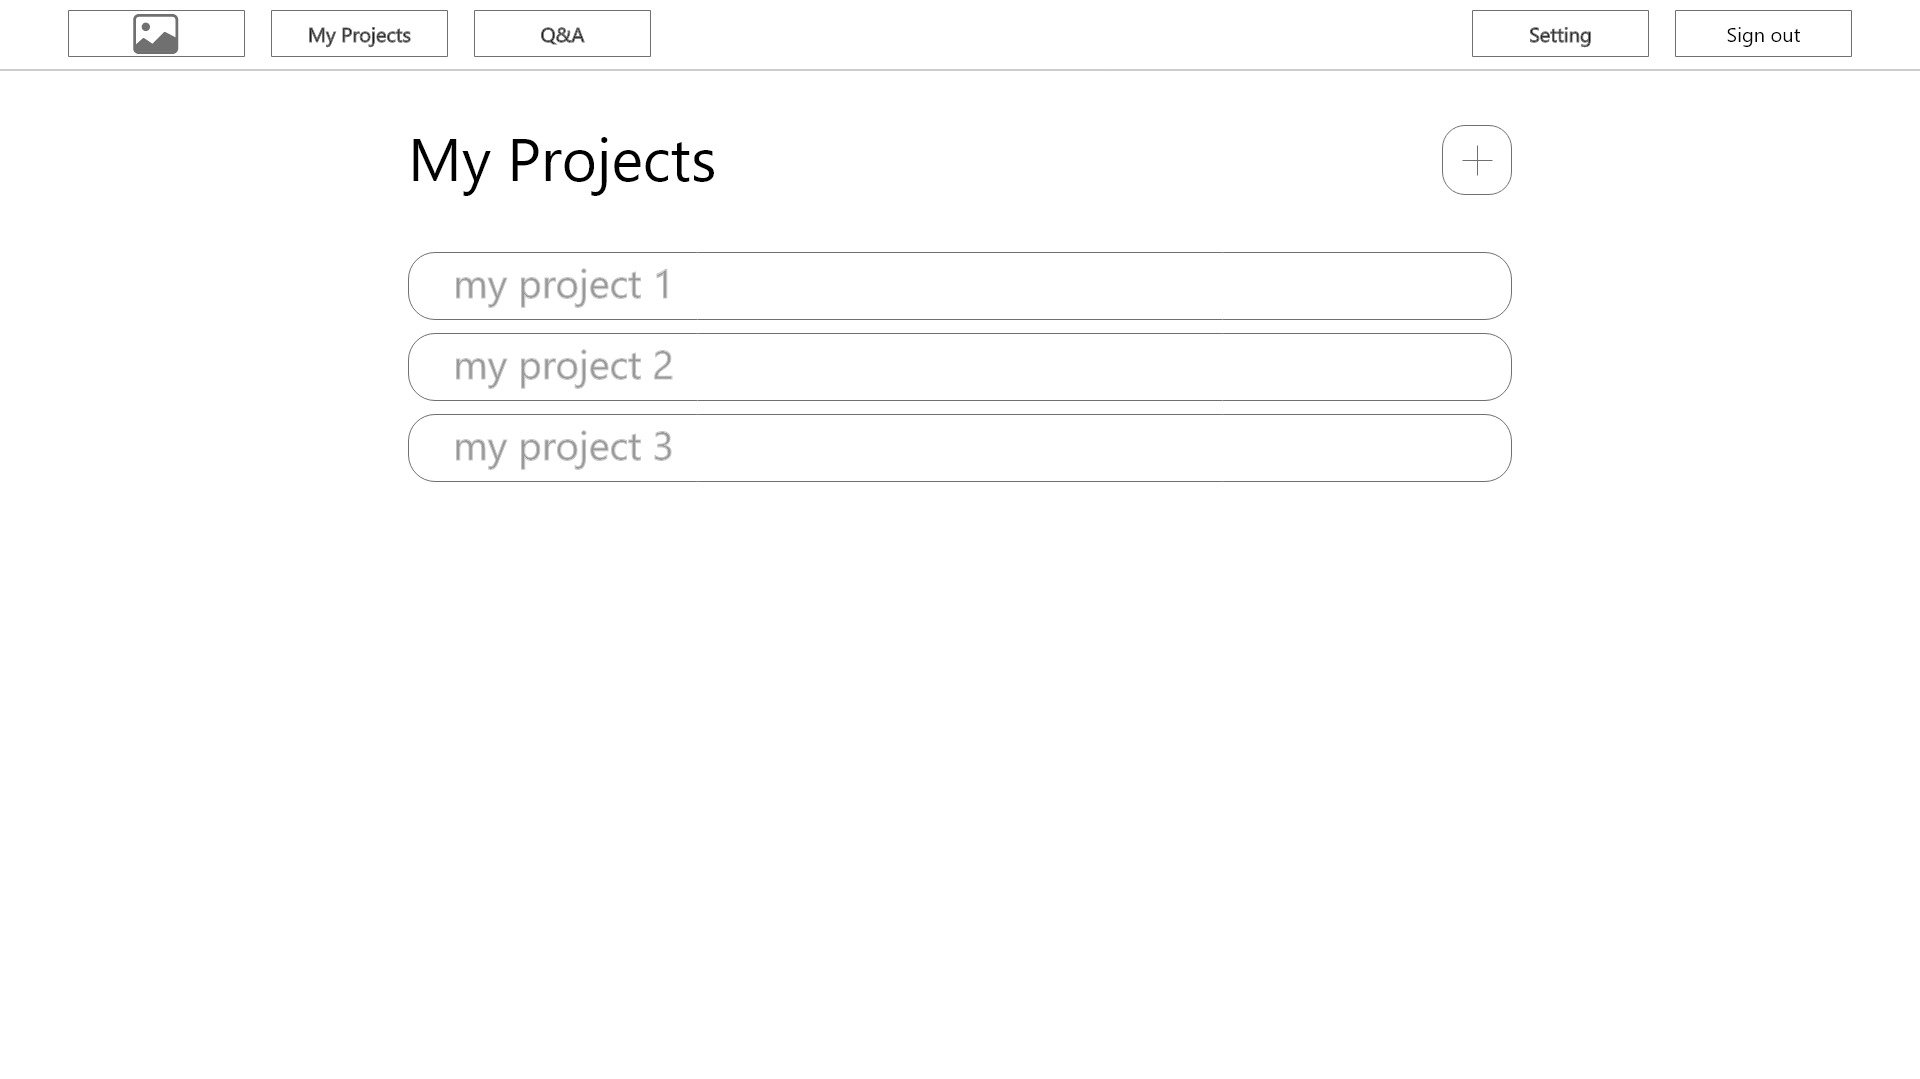
\includegraphics[width=\textwidth]{assets/wireframe/My_Projects.png}
  \item 專案初始化: 小林將自己的第一個專案命名為dian,並將專案設成Public,讓大家都能看見自己的專案,並加入README方便第一次進入專案的人,可以瞭解這個專案在做什麼和使用的流程。\\
  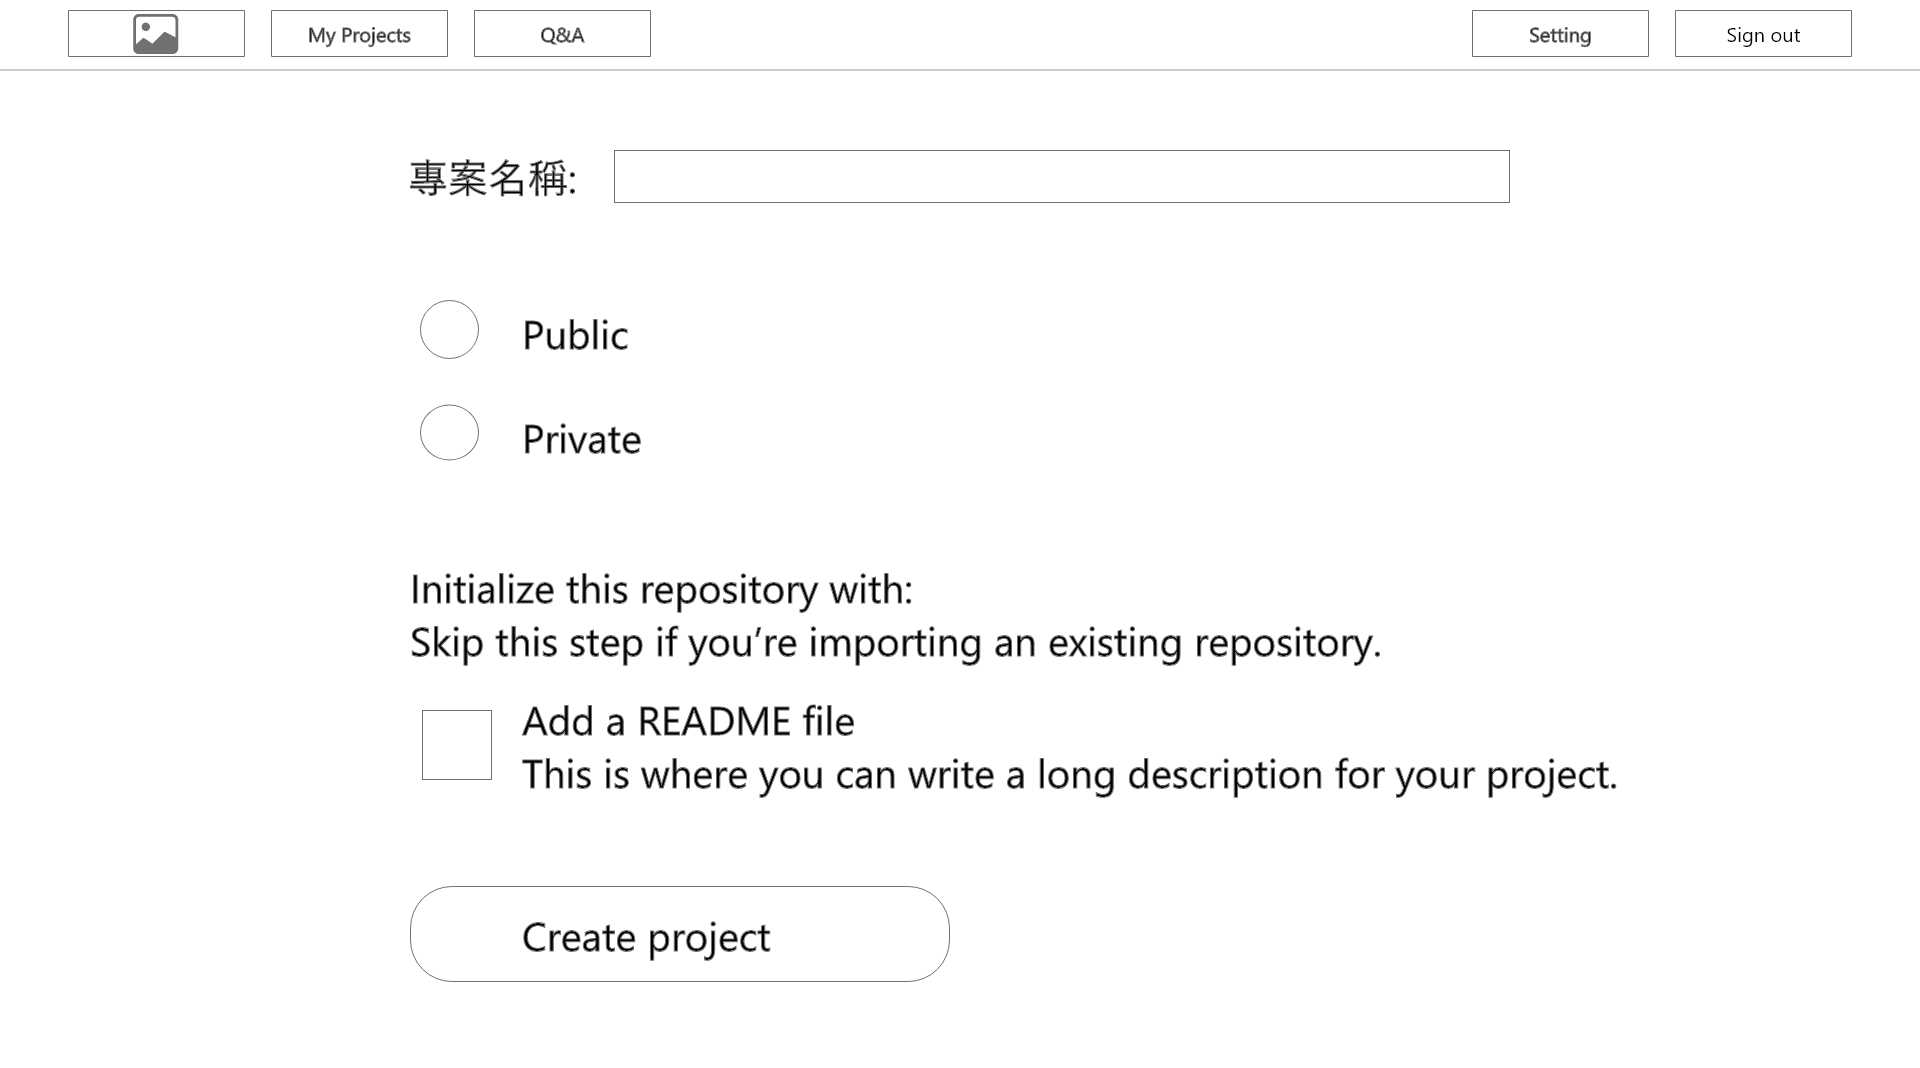
\includegraphics[width=\textwidth]{assets/wireframe/init_project.png}
  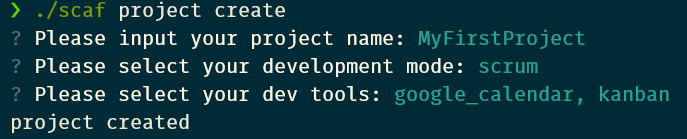
\includegraphics[width=\textwidth]{assets/wireframe/init_project_CLI.png}
  \item 建立repository: 小林因為想將前端和後端分開來放,所以按下new repository,建立兩個repository,repository3拿來放其他資料,分別在裡面放置前端和後端的檔案。\\
  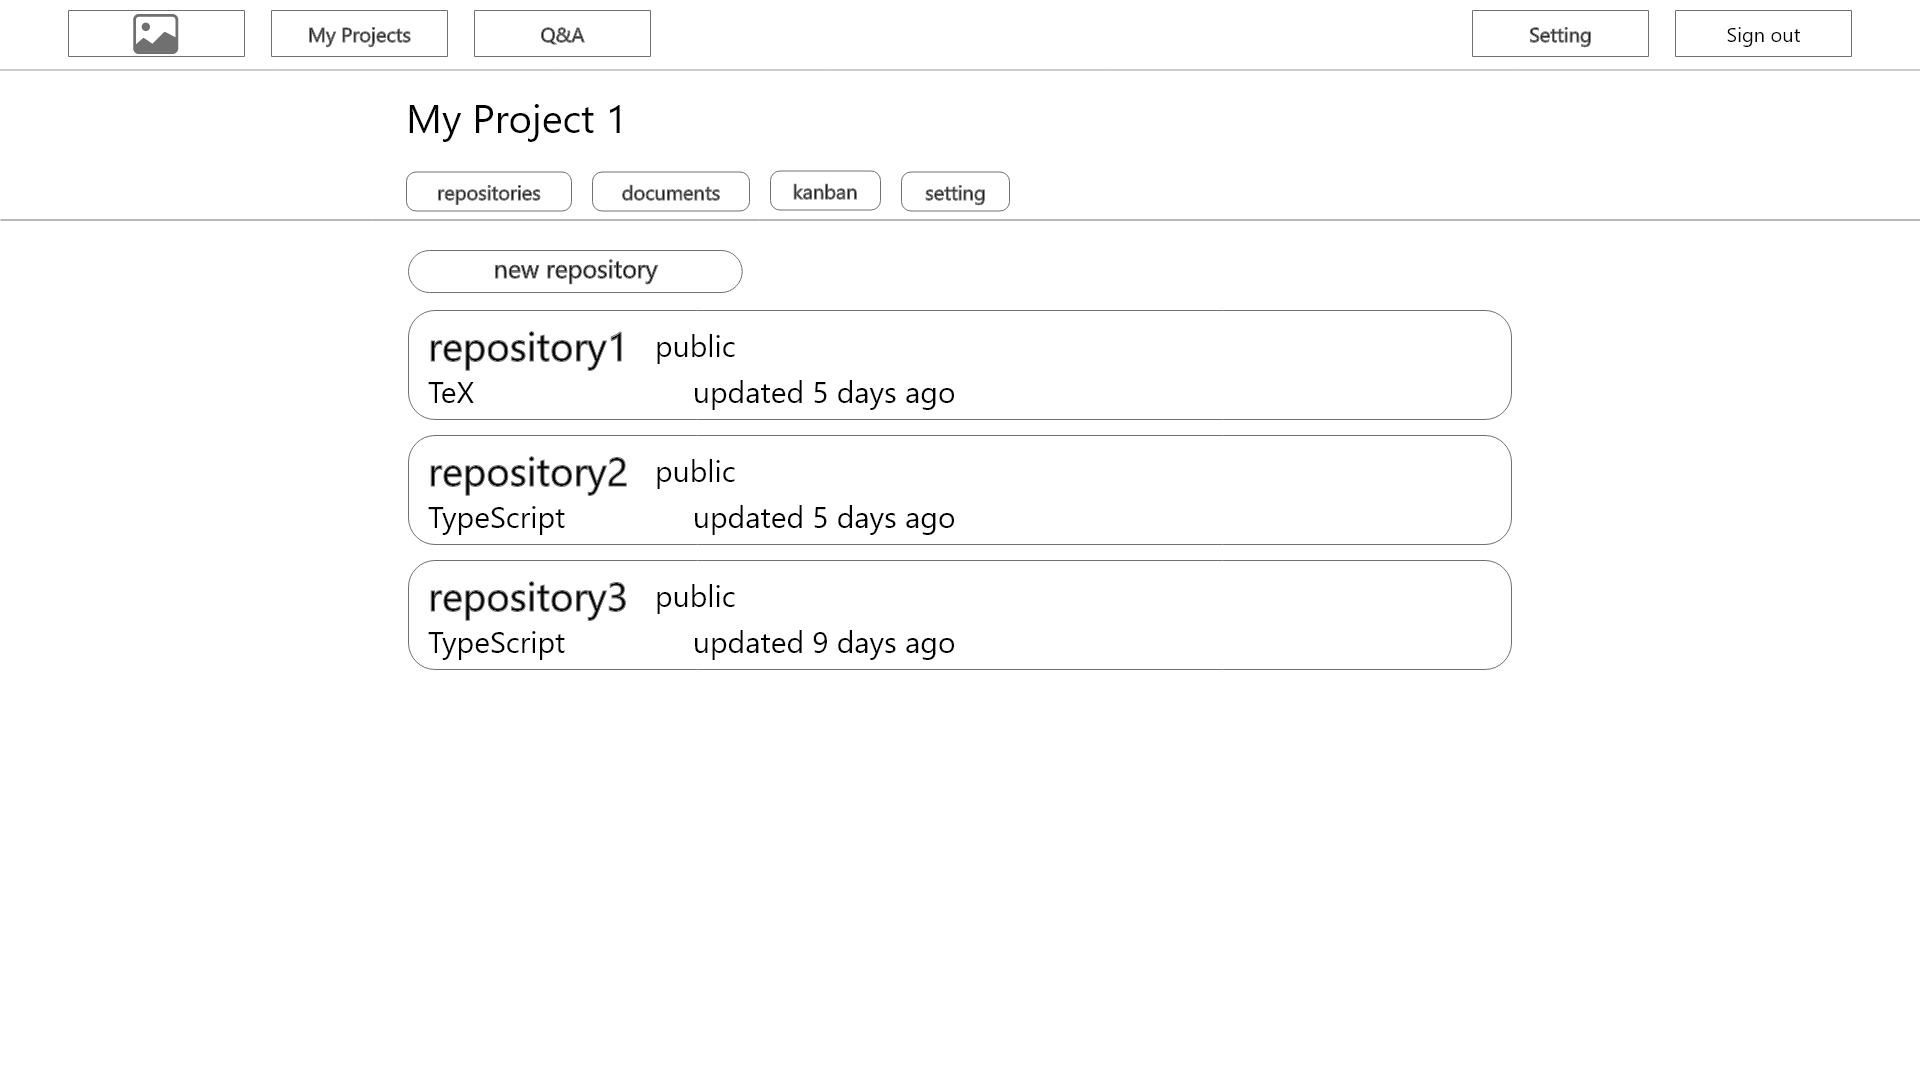
\includegraphics[width=\textwidth]{assets/wireframe/My_Projects_repositories.png}
  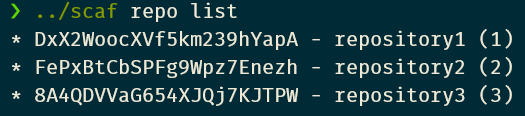
\includegraphics[width=\textwidth]{assets/wireframe/My_Projects_repositories_CLI.png}
  \item 在repository新增file: 小林使用HTML建立好了頁面的基本框架,repository1中可以點擊Add file,將自己的檔案上傳到網頁上。\\
  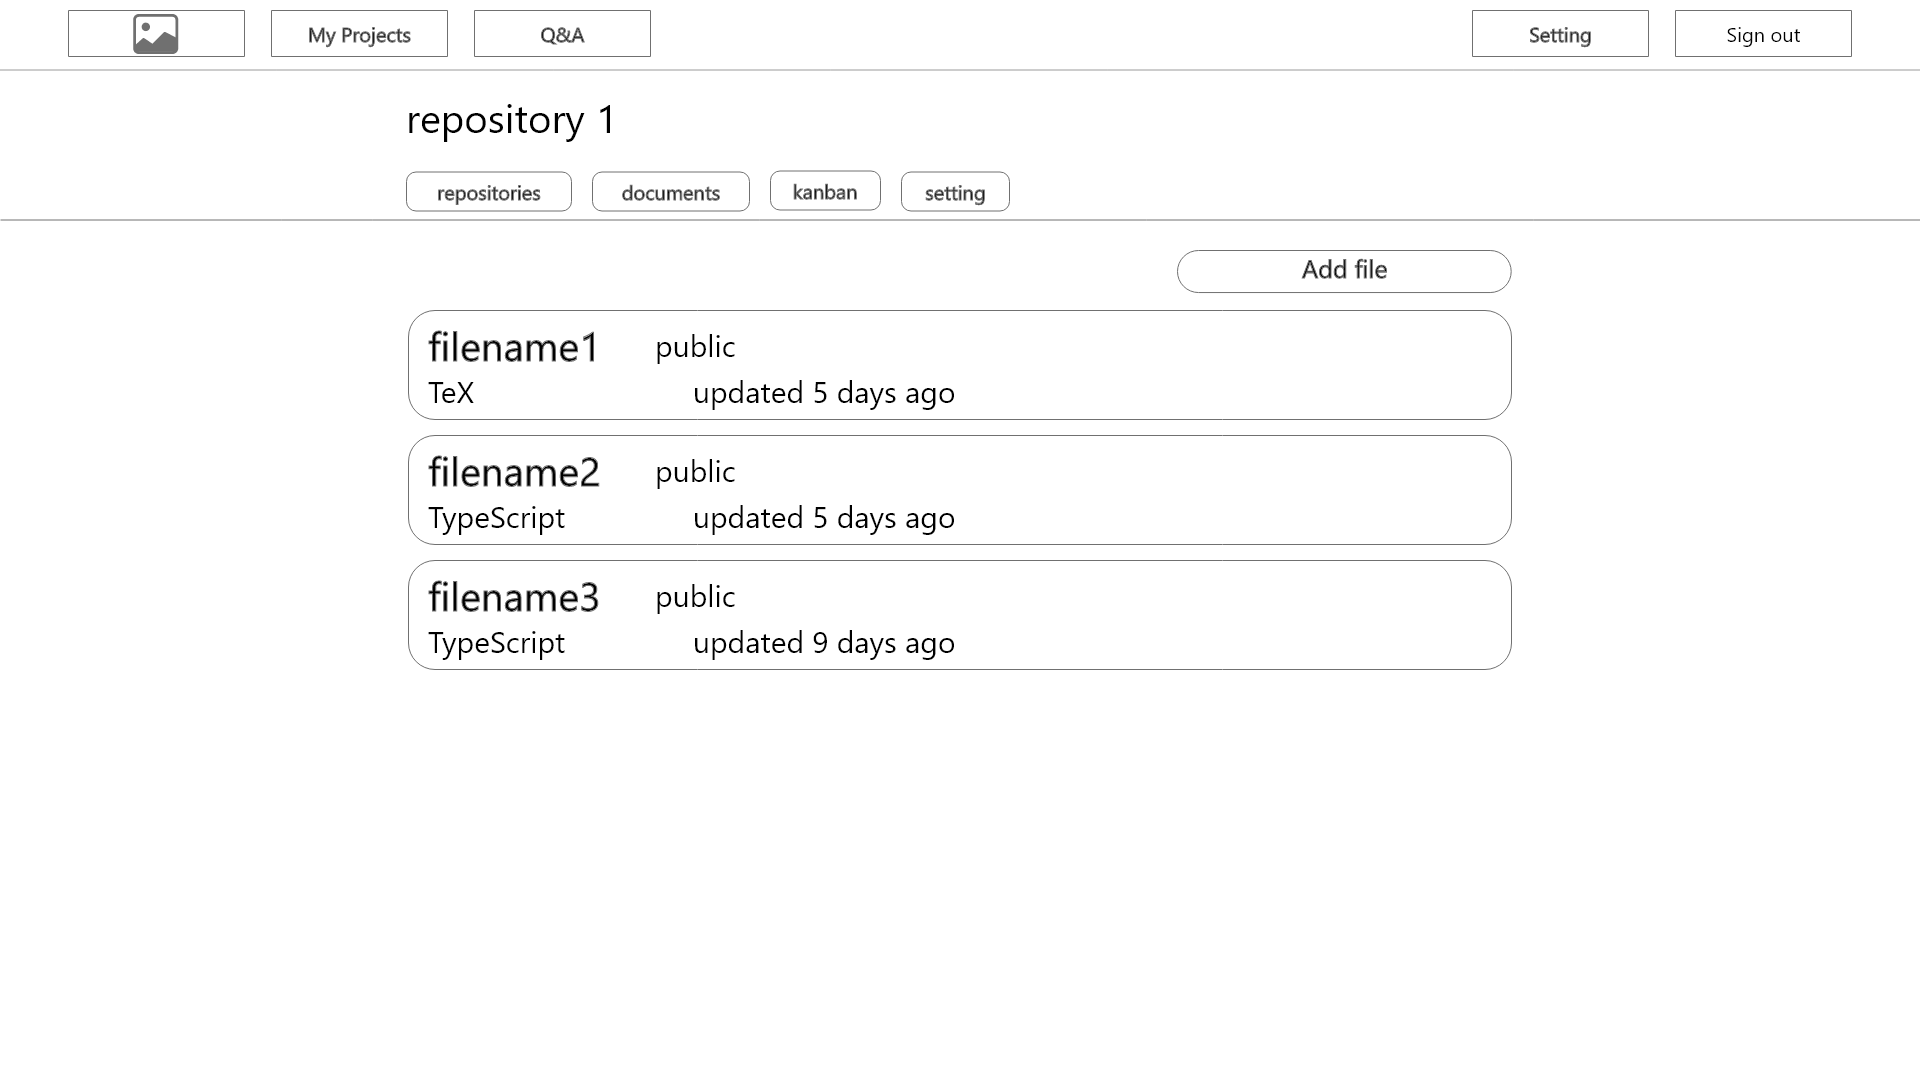
\includegraphics[width=\textwidth]{assets/wireframe/My_projects_add_file.png }
  \item 需求、設計、開發環境設定、命名規範、git commit format文件: 小林現在想要來建立文件,於是他按下了documents,然後再document頁面中選擇需求文件,並按下edit(若是檔案已經存在,會顯示預覽畫面)。\\
  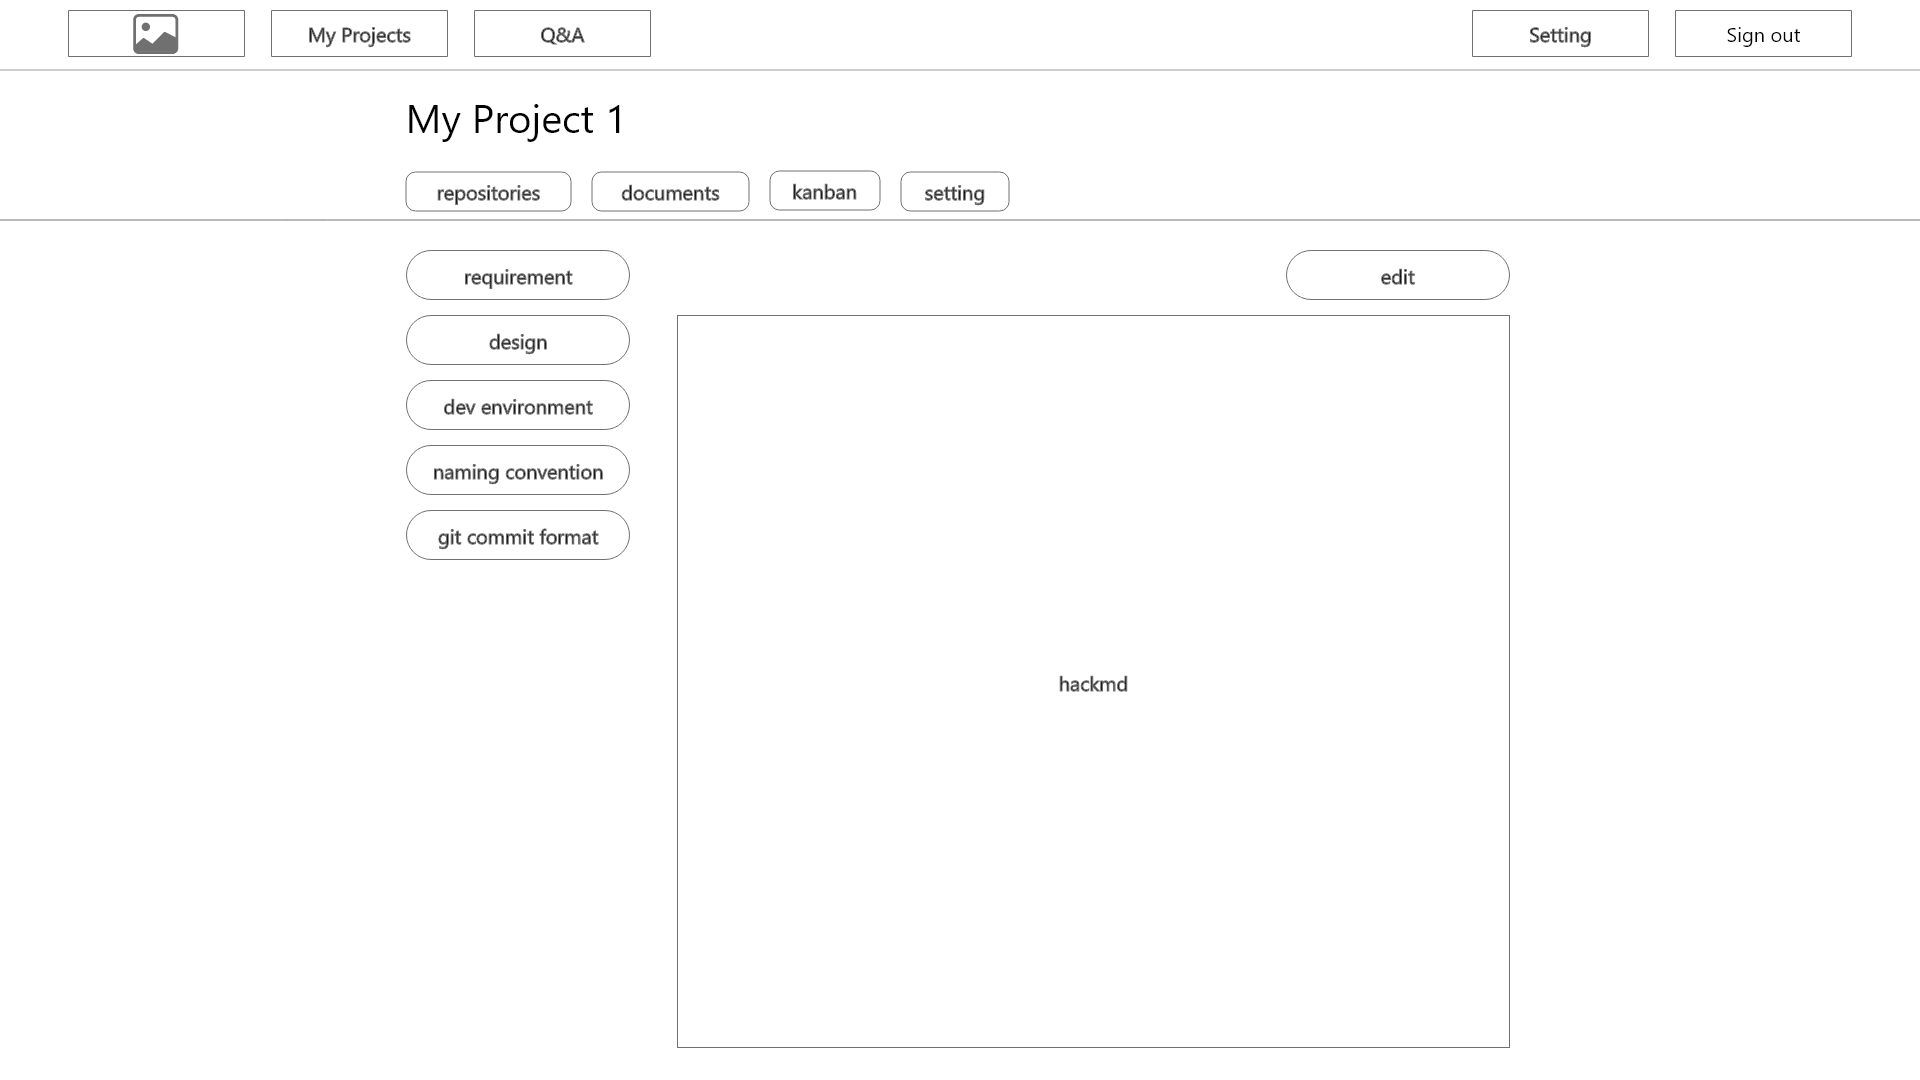
\includegraphics[width=\textwidth]{assets/wireframe/My_Projects_documents_requirement_dev_environment_naming_convention_git commit format.png }
  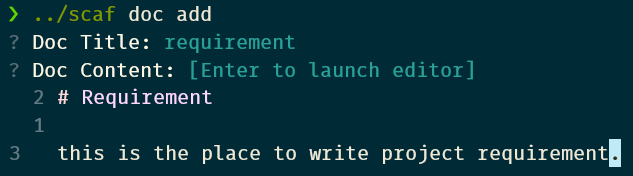
\includegraphics[width=\textwidth]{assets/wireframe/My_Projects_documents_requirement_dev_environment_naming_convention_git commit format_CLI.png }
  \item hackmd: 小林進入到hackmd中編輯需求文件。\\
  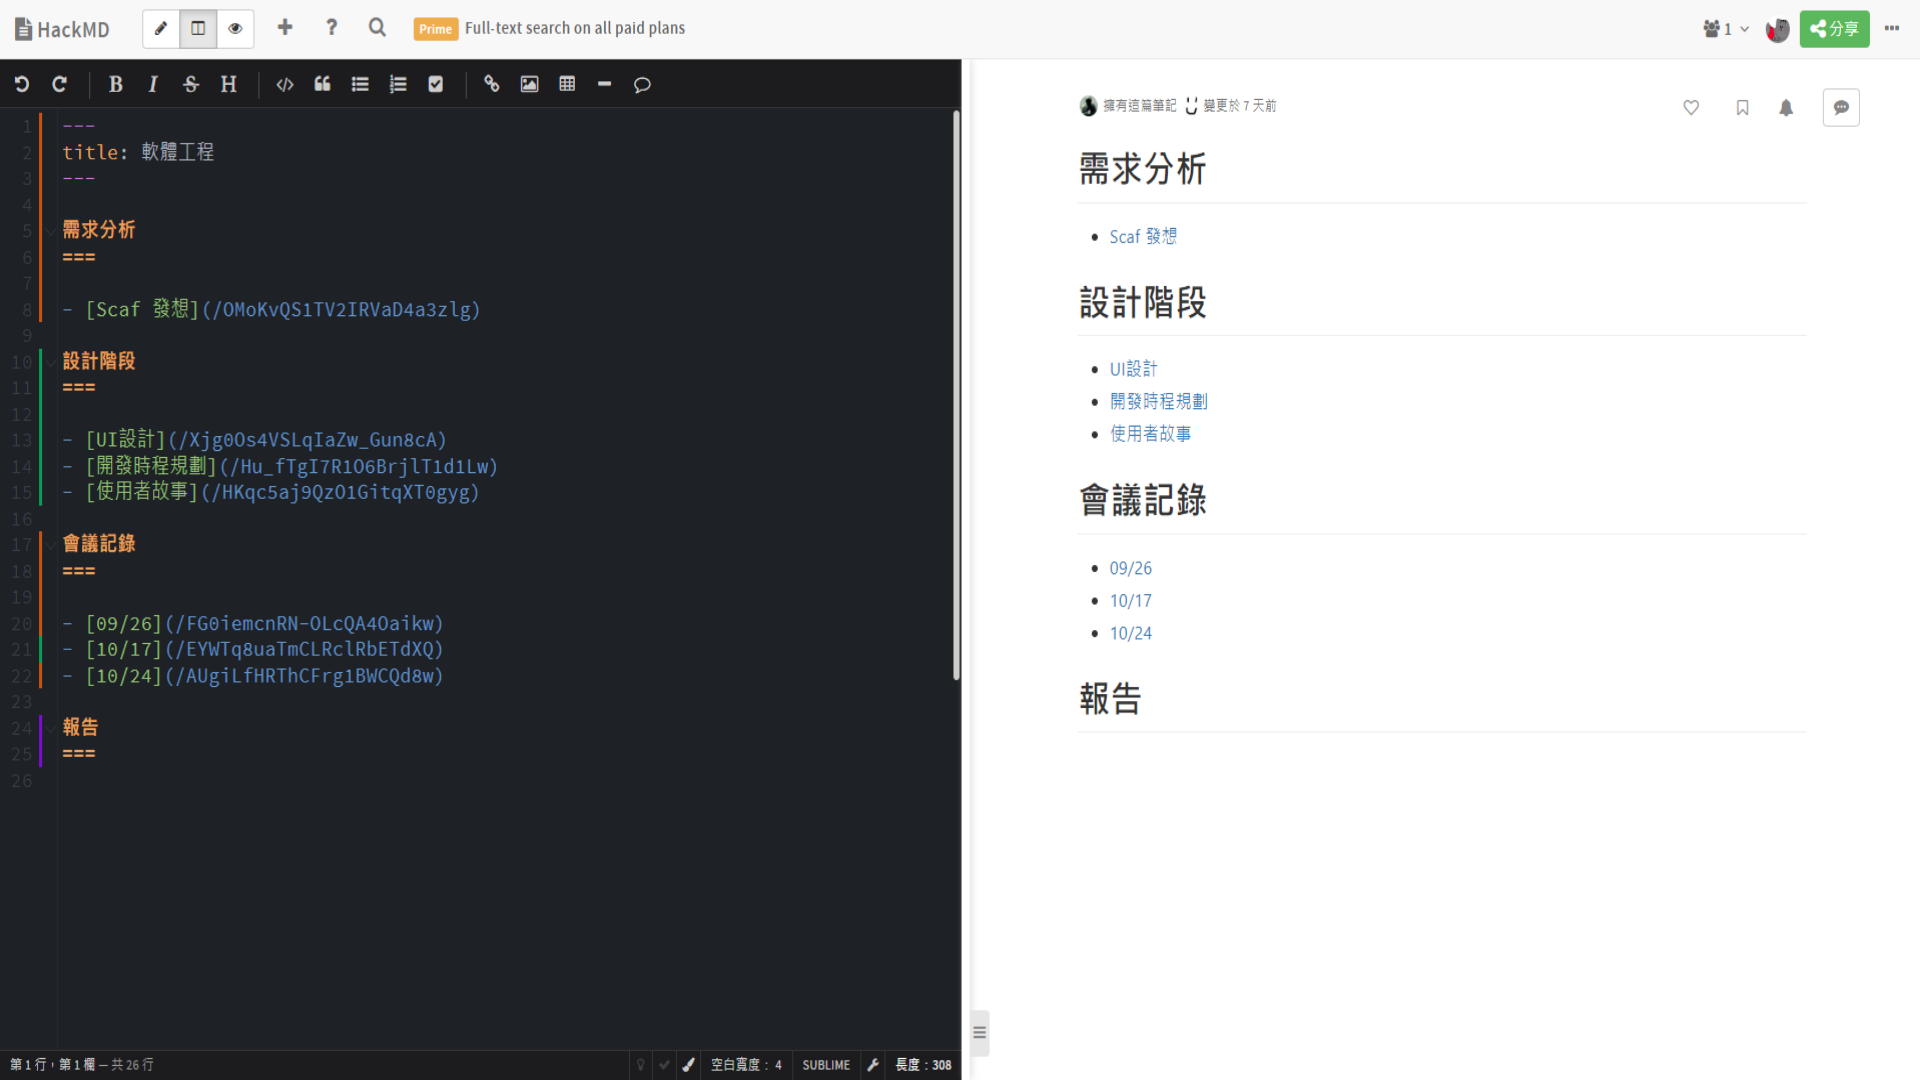
\includegraphics[width=\textwidth]{assets/wireframe/hackmd.png}
  \item 看板: 小林這時想記錄每個工作的完成進度,於是點擊kanban按鈕進入到kanban頁面,按下New task建立新的task,並設定任務標籤、任務描述、deadline與分配負責成員。\\
  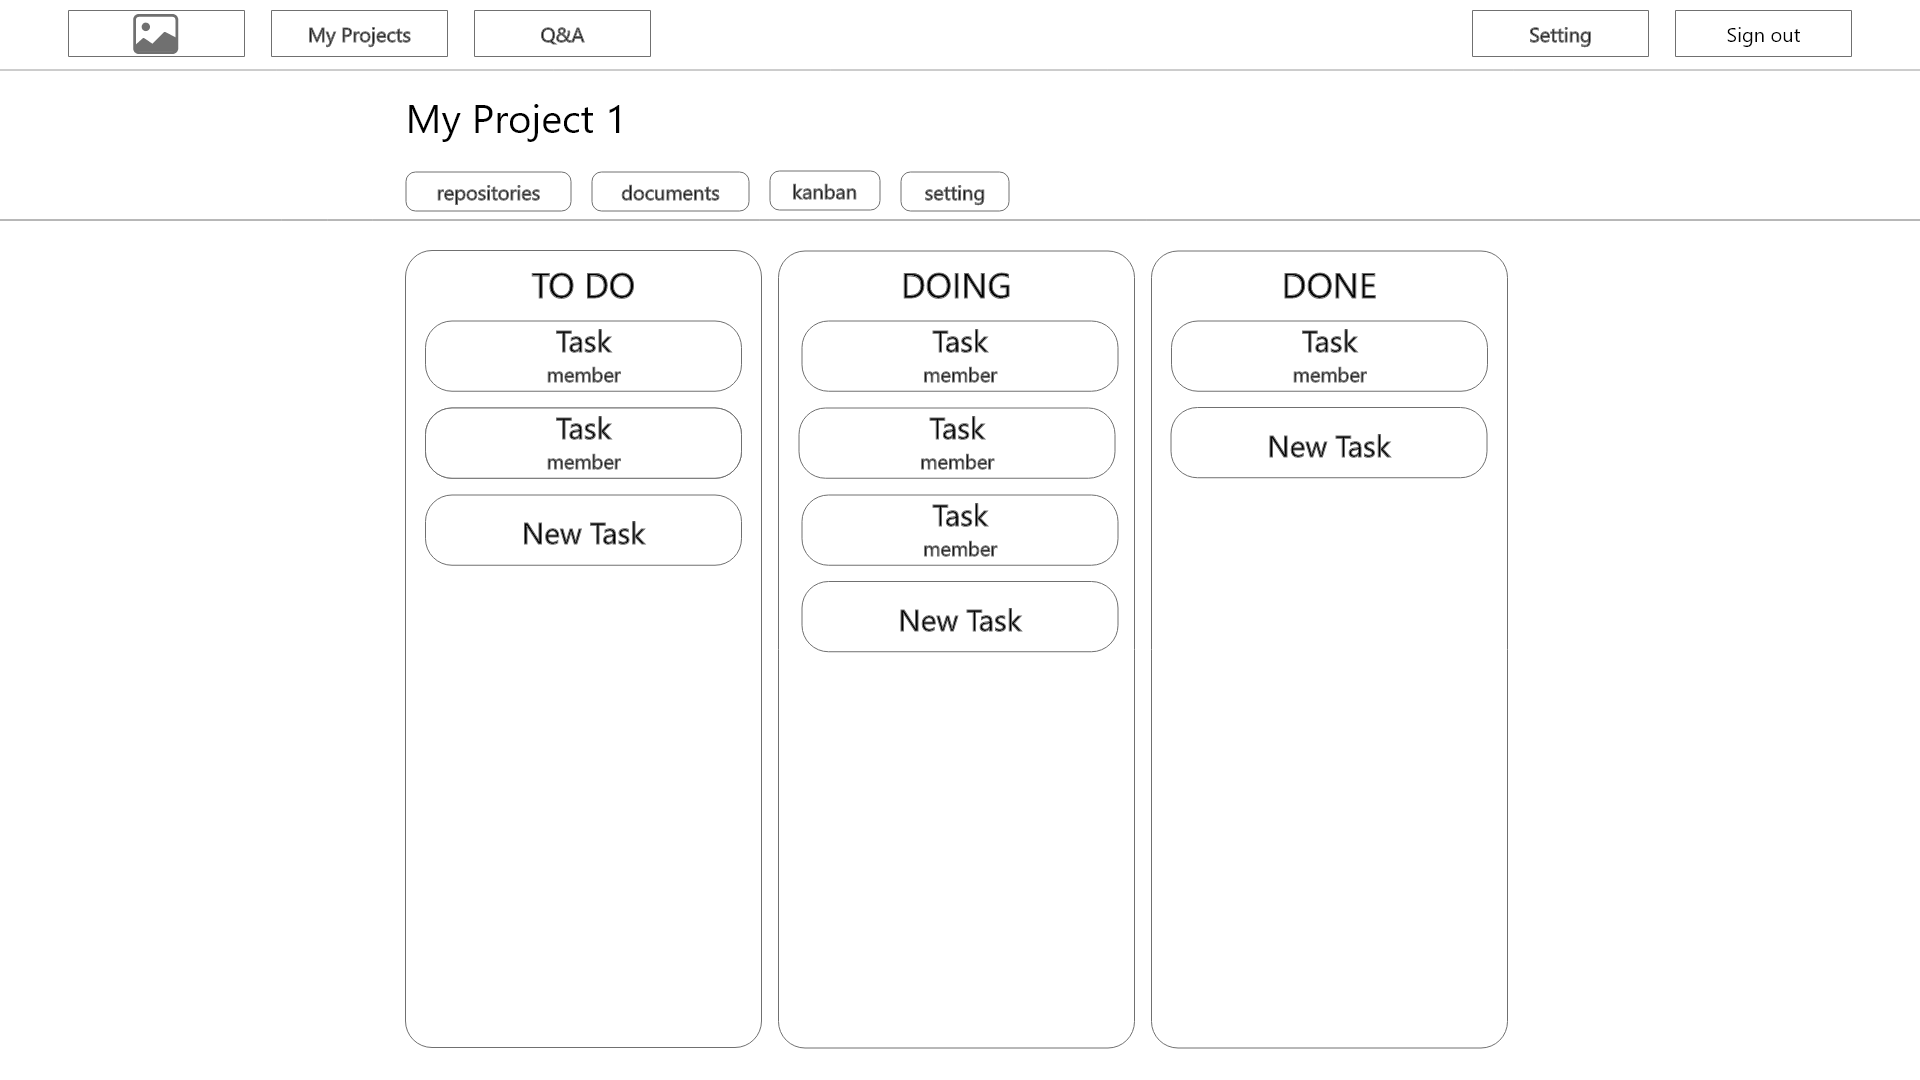
\includegraphics[width=\textwidth]{assets/wireframe/My_Projects_kanban.png}
  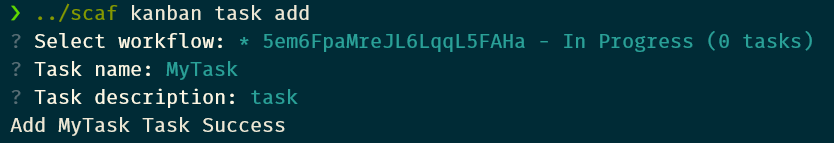
\includegraphics[width=\textwidth]{assets/wireframe/My_Projects_kanban_CLI.png}
  \item 更改專案名稱: 小林這時發現自己的專案名稱太中二了,於是按下setting按鈕(project bar)進入到setting頁面,並點選general去更新自己的專案名稱。\\
  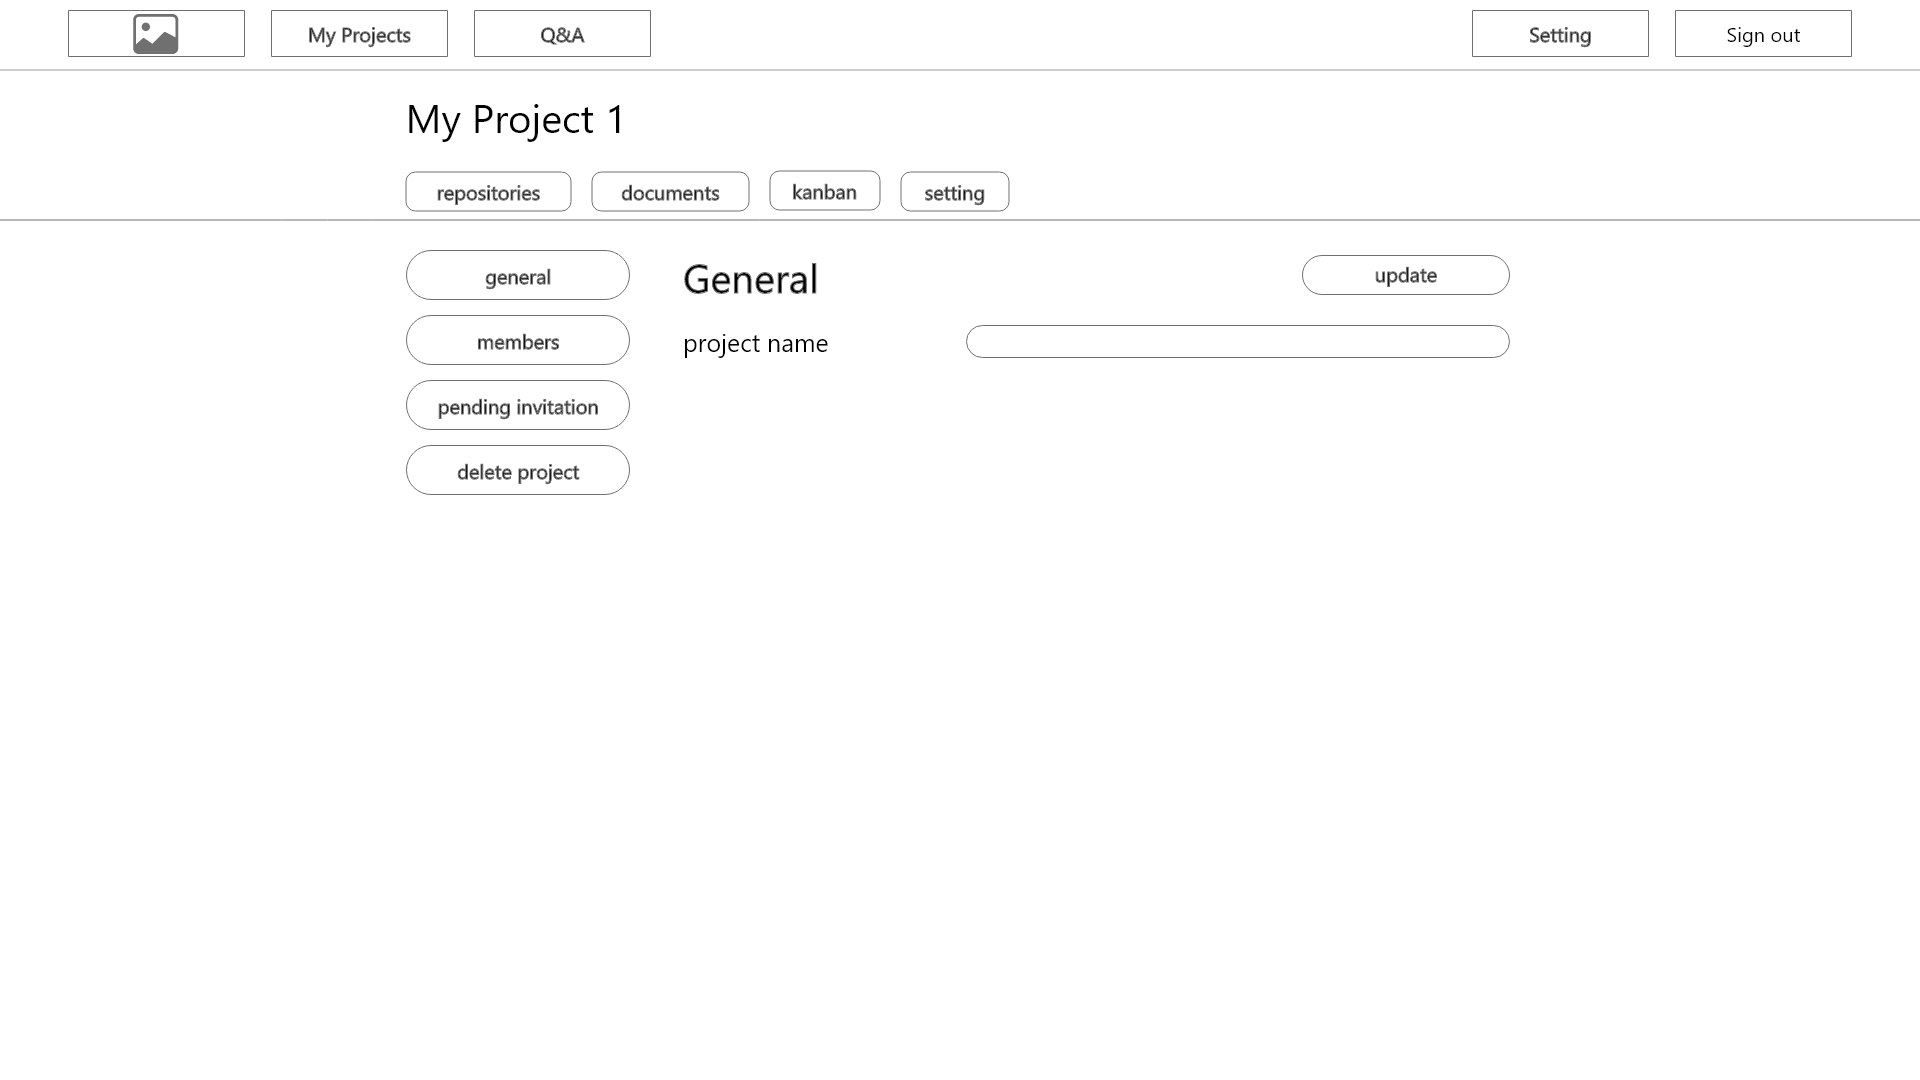
\includegraphics[width=\textwidth]{assets/wireframe/My_Projects_setting_general.png}
  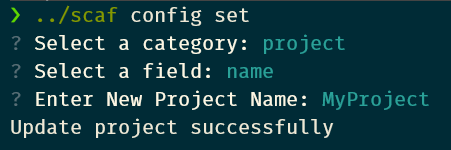
\includegraphics[width=\textwidth]{assets/wireframe/My_Projects_setting_general_CLI.png}
  \item 變更專案成員: 小林因為發現自己的組員都在耍廢,好像做完這份專案分錢的人太多了,於是他按下setting把所有人都踢出了,並按下invite邀請了一個大腿。\\
  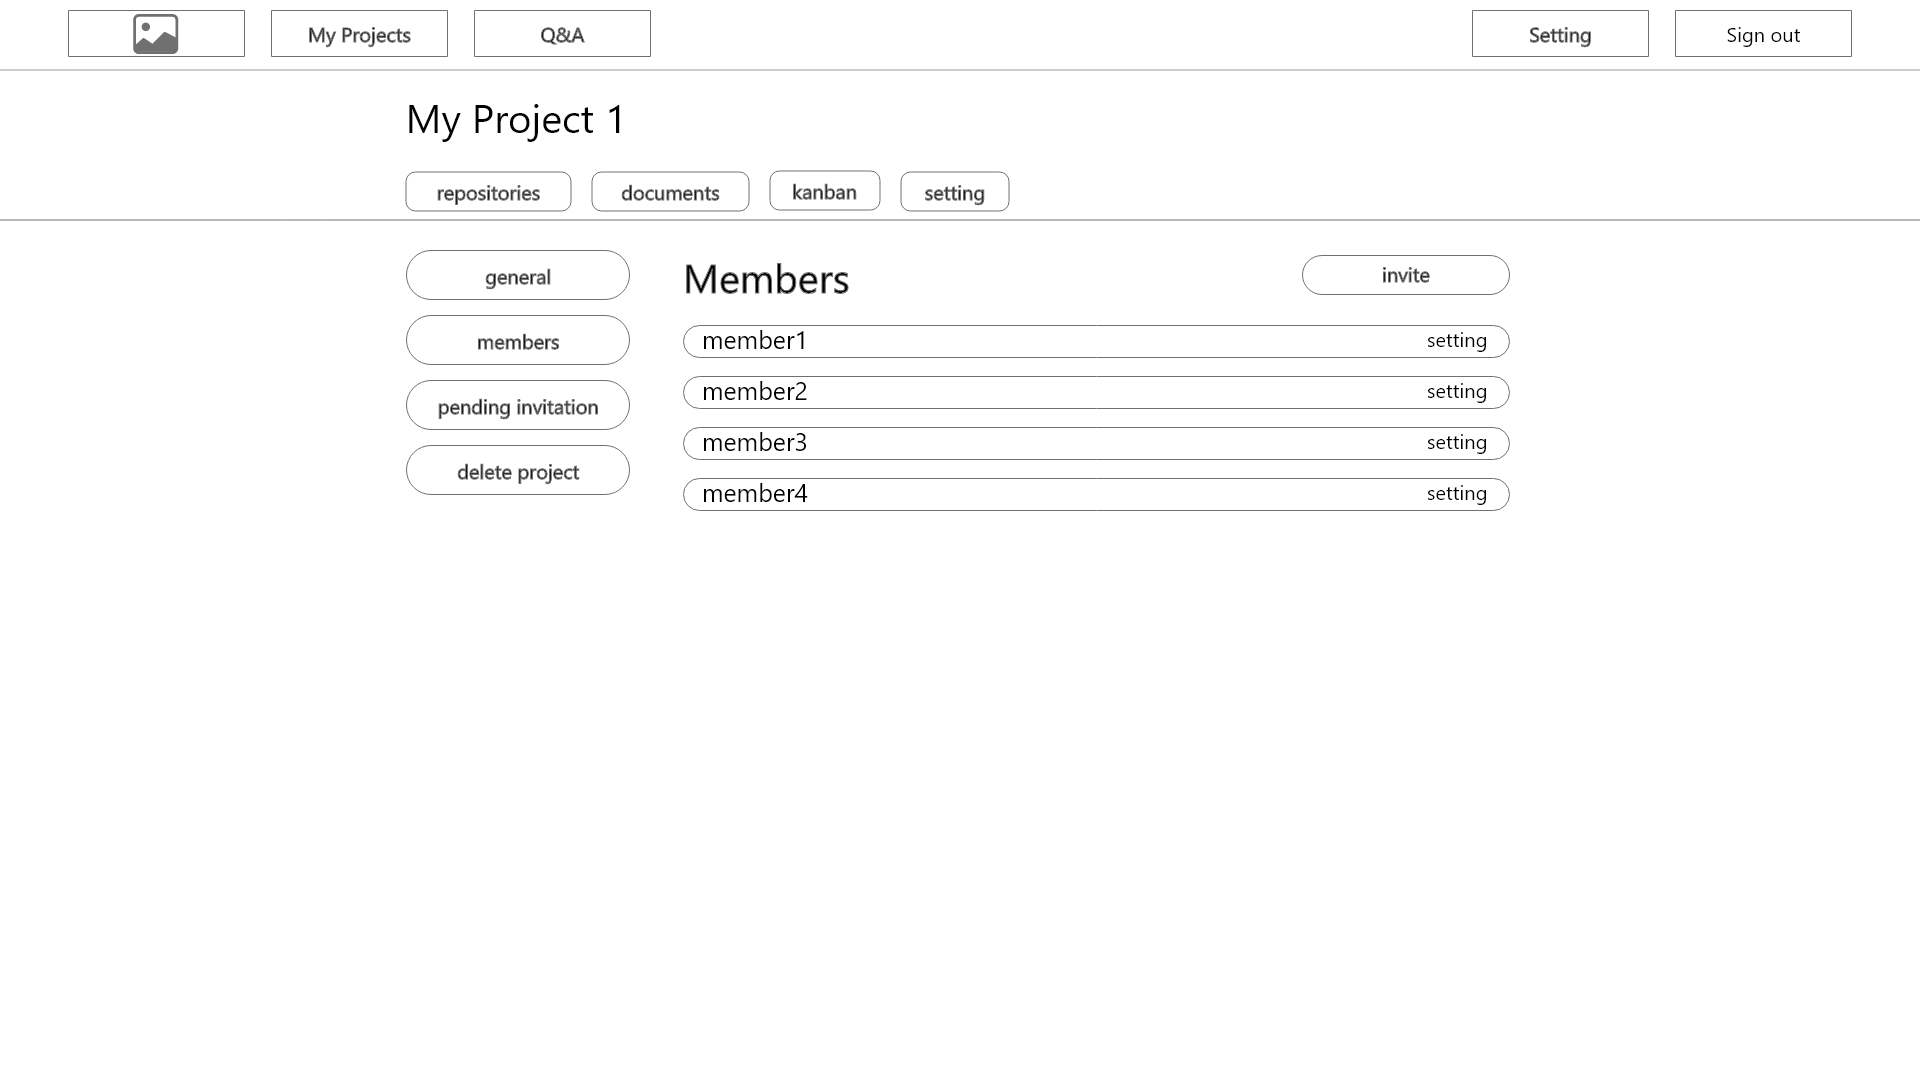
\includegraphics[width=\textwidth]{assets/wireframe/My_Projects_setting_members.png}
  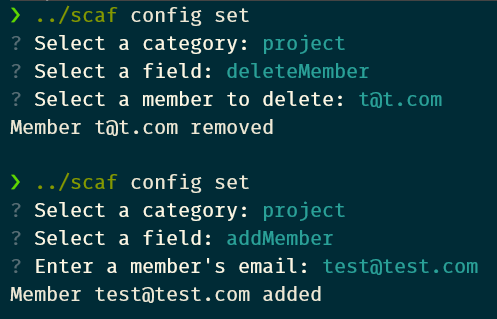
\includegraphics[width=\textwidth]{assets/wireframe/My_Projects_setting_members_CLI.png}
  \item 處理加入專案申請: 小林覺得自己的專案很牛逼,於是想看看有沒有人提出申請加入專案,按下了pending invitation來看看有哪些有用的人,並按下YES確認了他們的申請。\\
  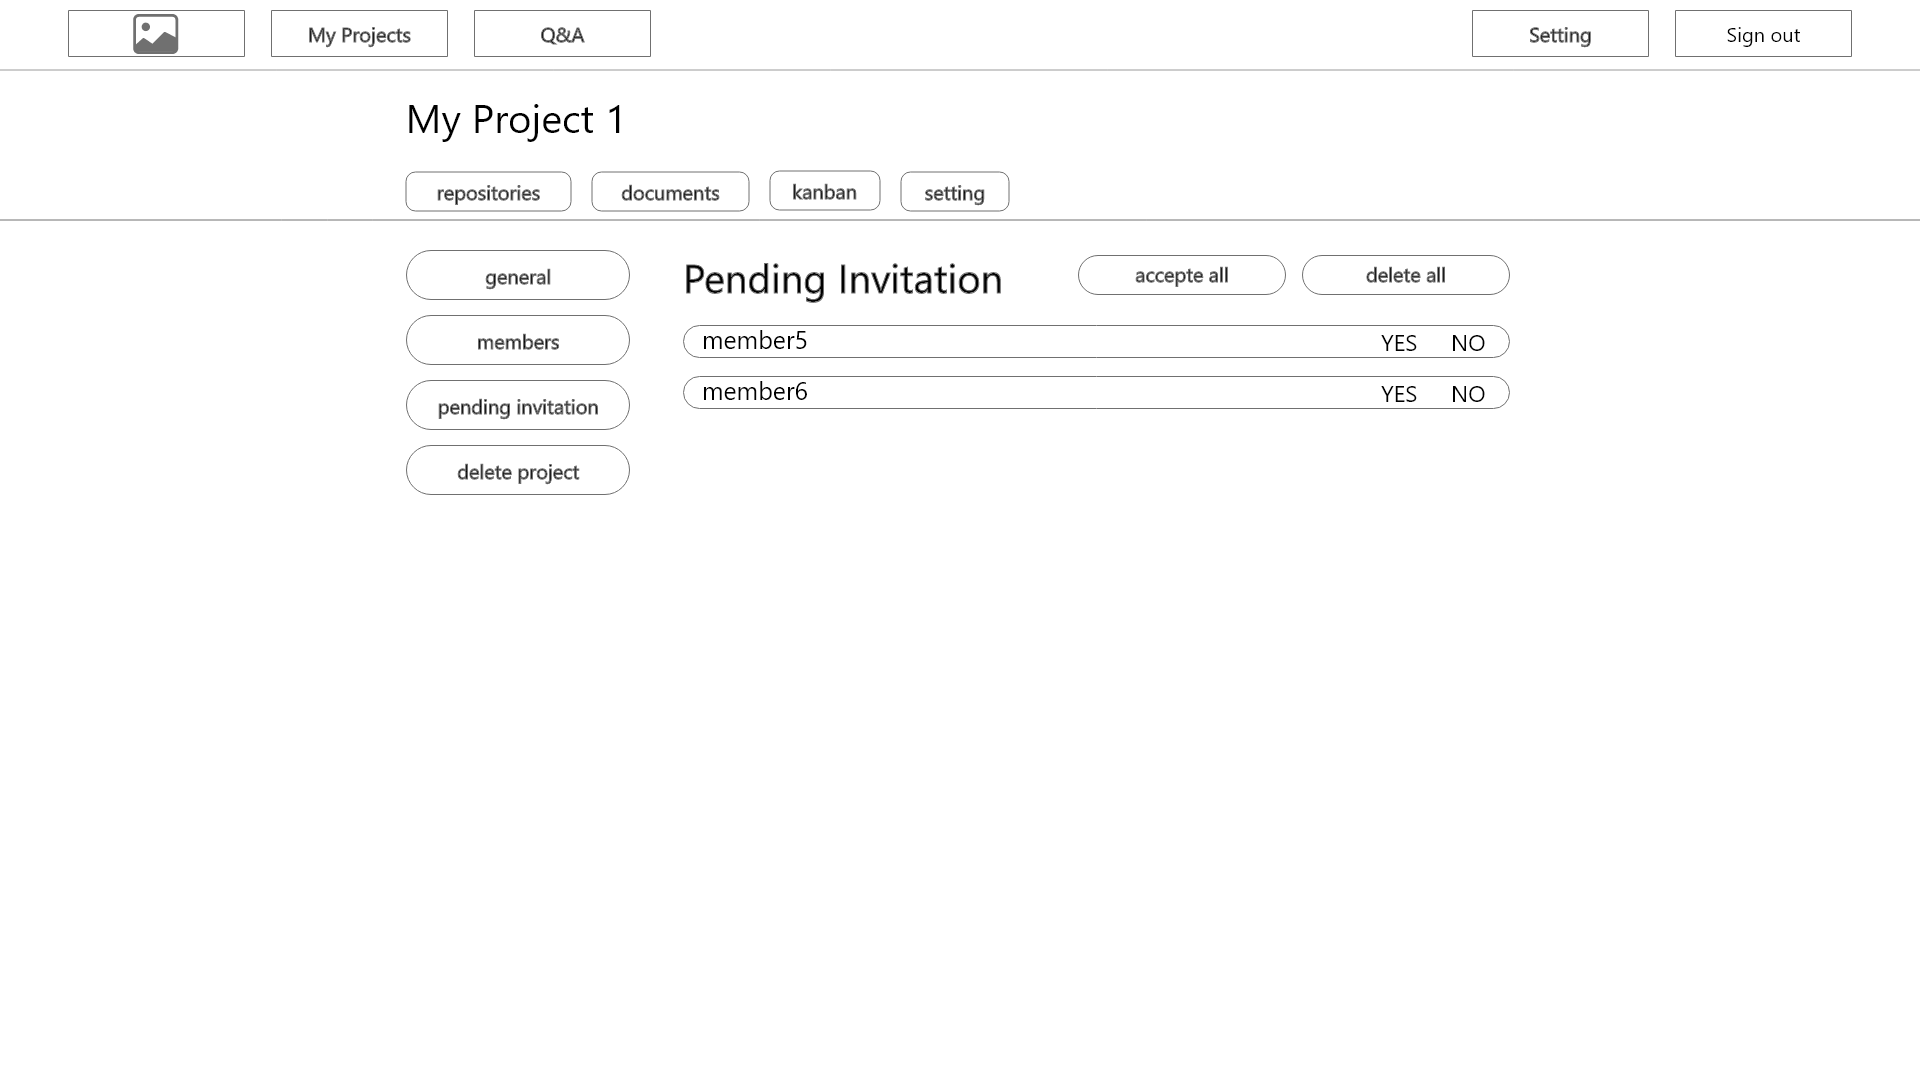
\includegraphics[width=\textwidth]{assets/wireframe/My_Projects_setting_pending_invitation.png}
  \item 刪除專案: 小林覺得這個專案真的是太麻煩了,於是按下了delete project把整個專案給刪除了。\\
  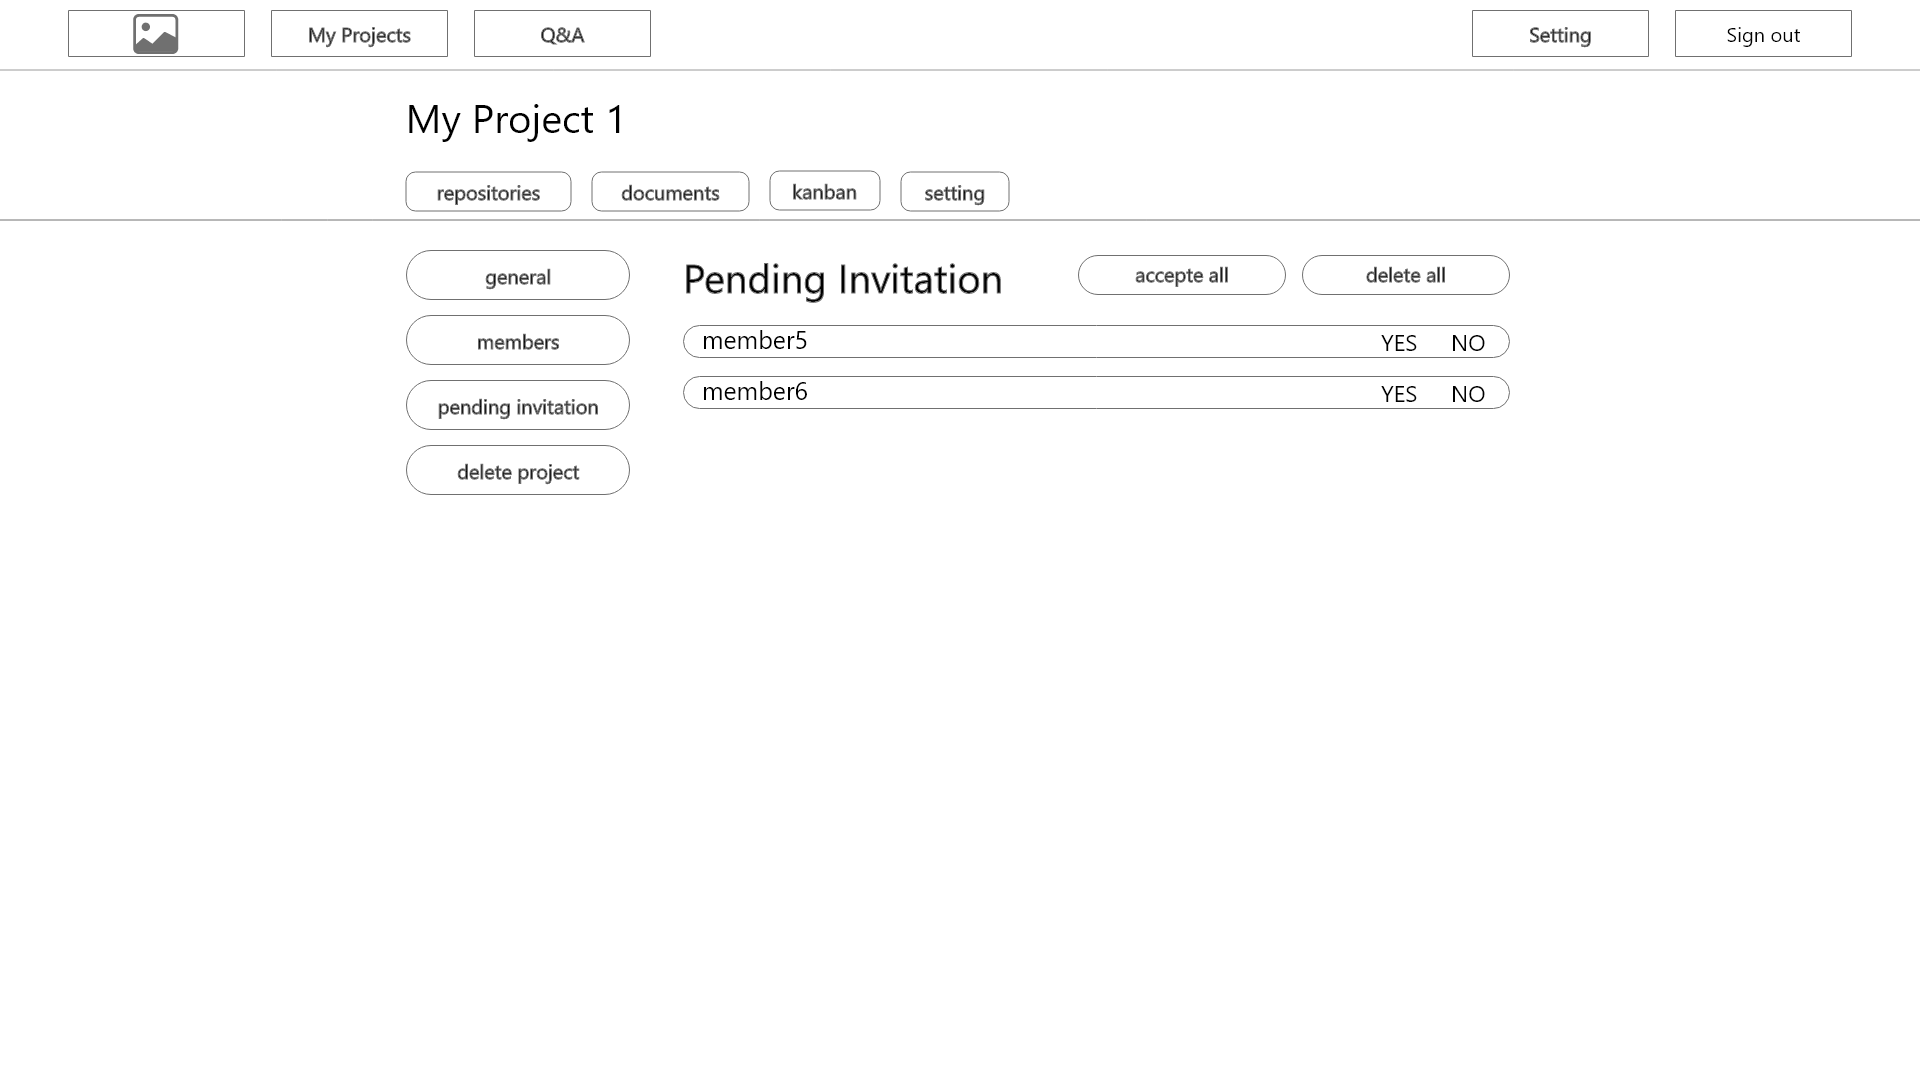
\includegraphics[width=\textwidth]{assets/wireframe/My_Projects_setting_pending_invitation.png}
  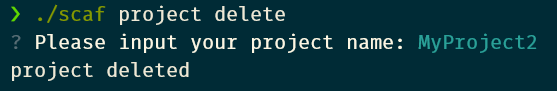
\includegraphics[width=\textwidth]{assets/wireframe/My_Projects_setting_delete_CLI.png}
  \item QA文件: 小林想要看看測試和部屬階段有沒有什麼常見的疑問,於是按下了QA,並按下testing or deployment。\\
  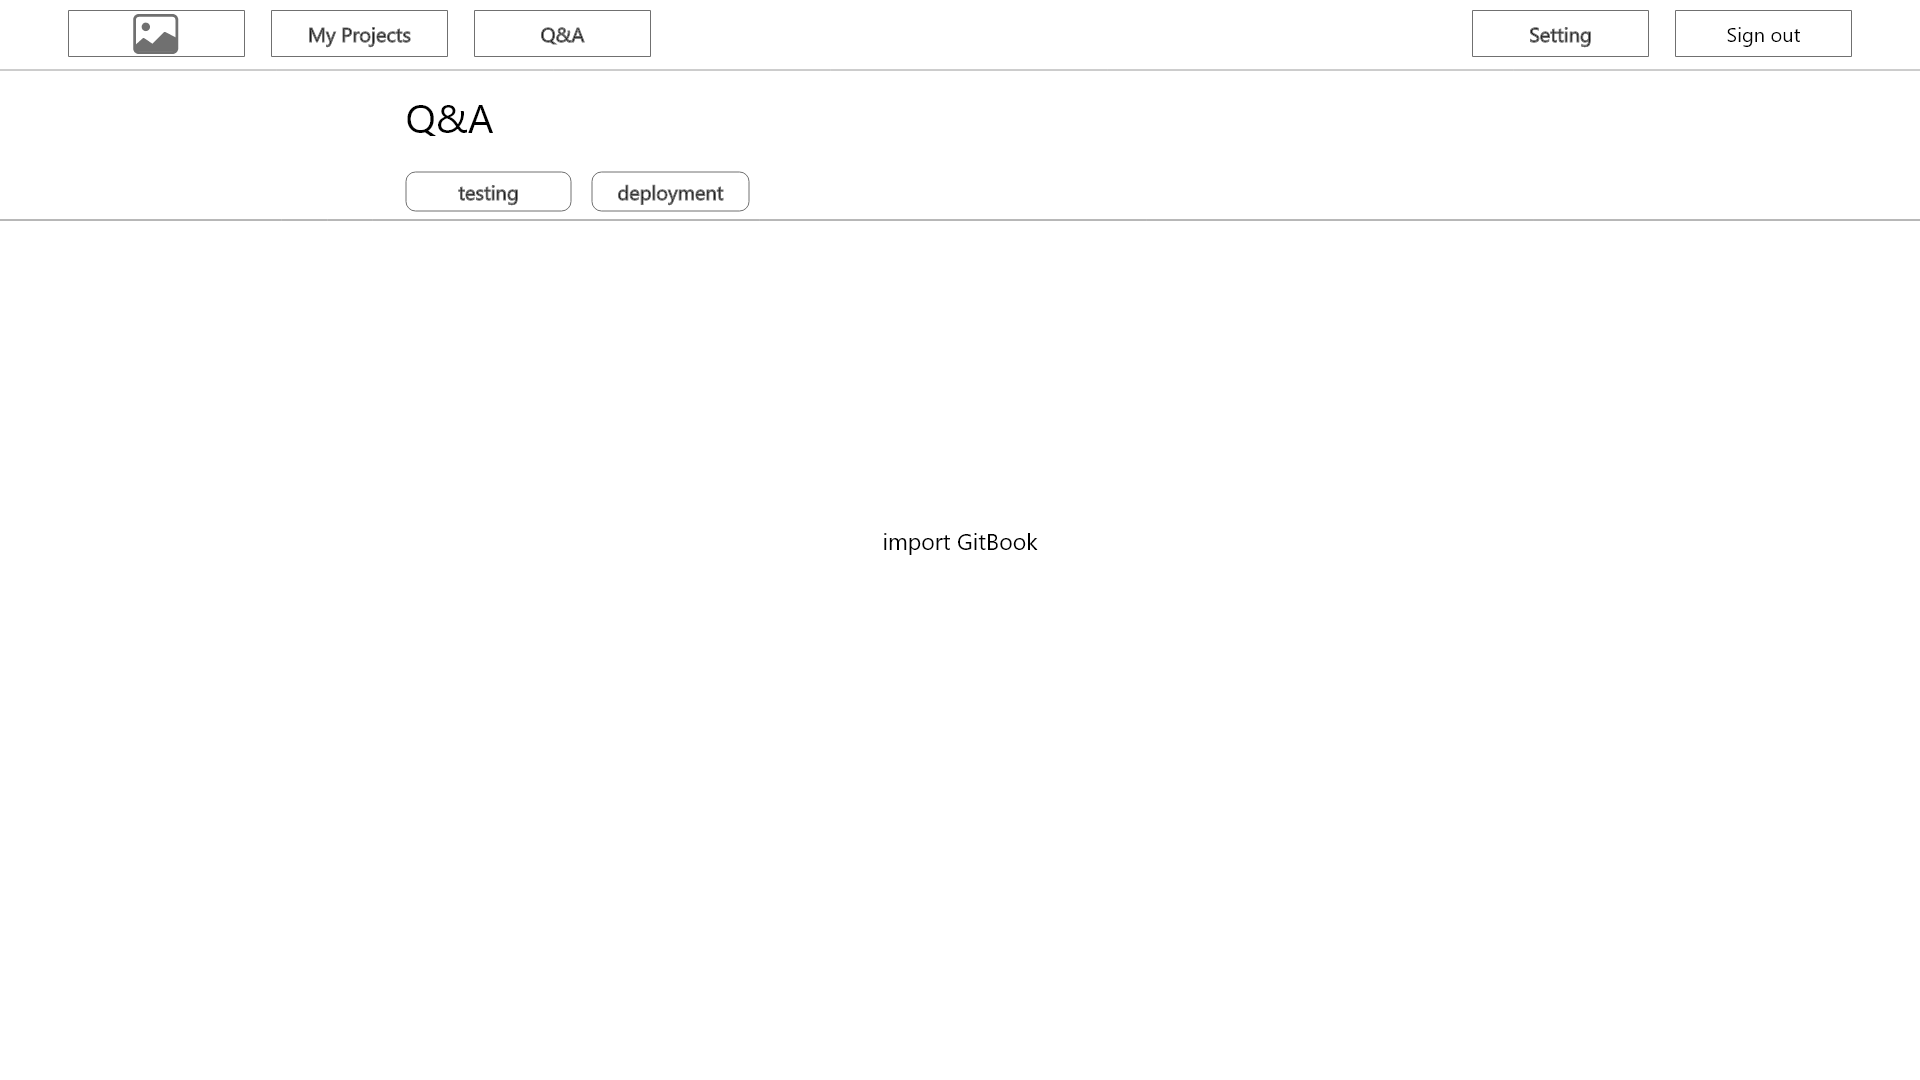
\includegraphics[width=\textwidth]{assets/wireframe/QA_testing_deployment.png}
  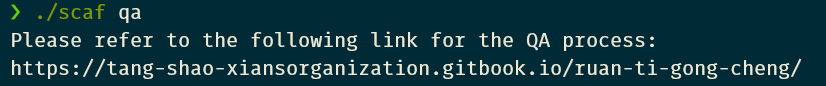
\includegraphics[width=\textwidth]{assets/wireframe/QA_testing_deployment_CLI.png}
  \item gitbook: 小林可以直接在下方的頁面中瀏覽gitbook。 \\
  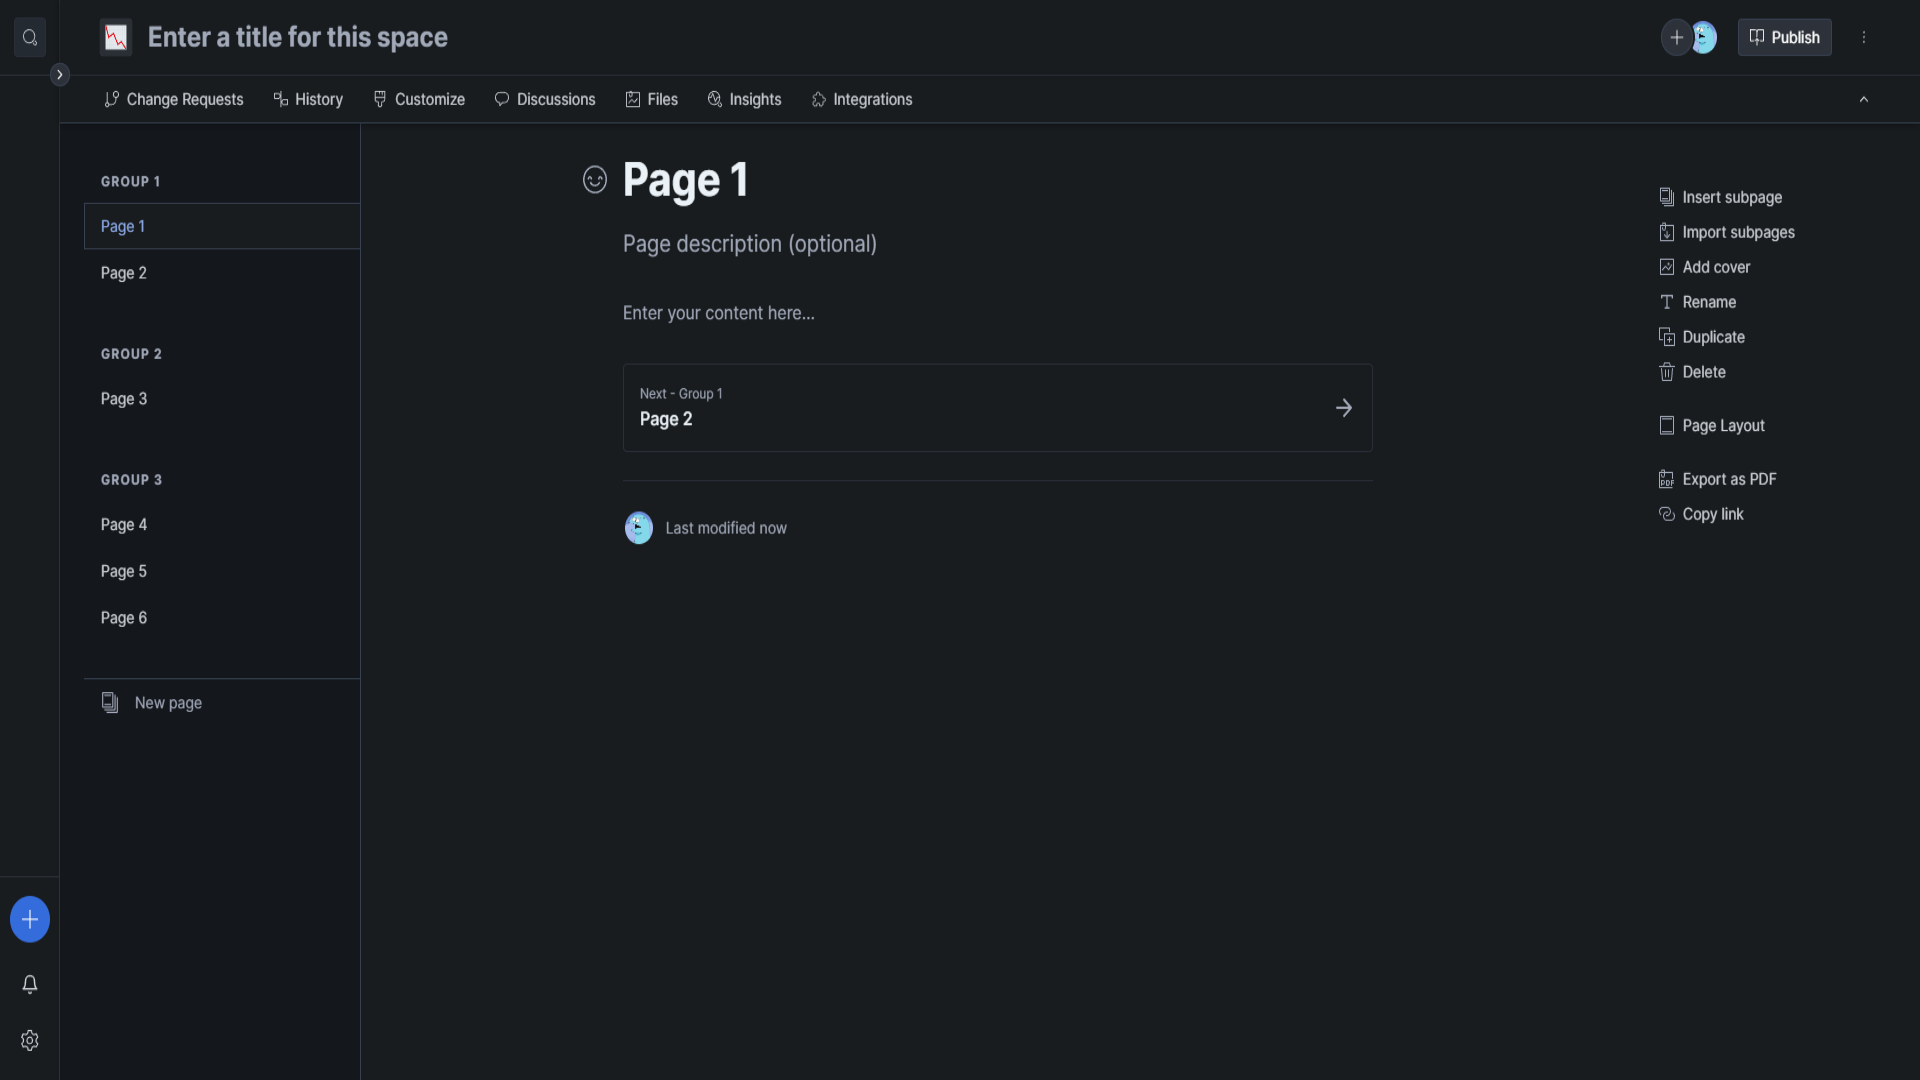
\includegraphics[width=\textwidth]{assets/wireframe/gitbook.png}
  \item 上傳自己的傳片: 小林覺得自己太帥了想要讓大家都看到自己的照片,所以按下了main bar中的setting按鈕,並按下ADD your photo新增自己的照片。\\
  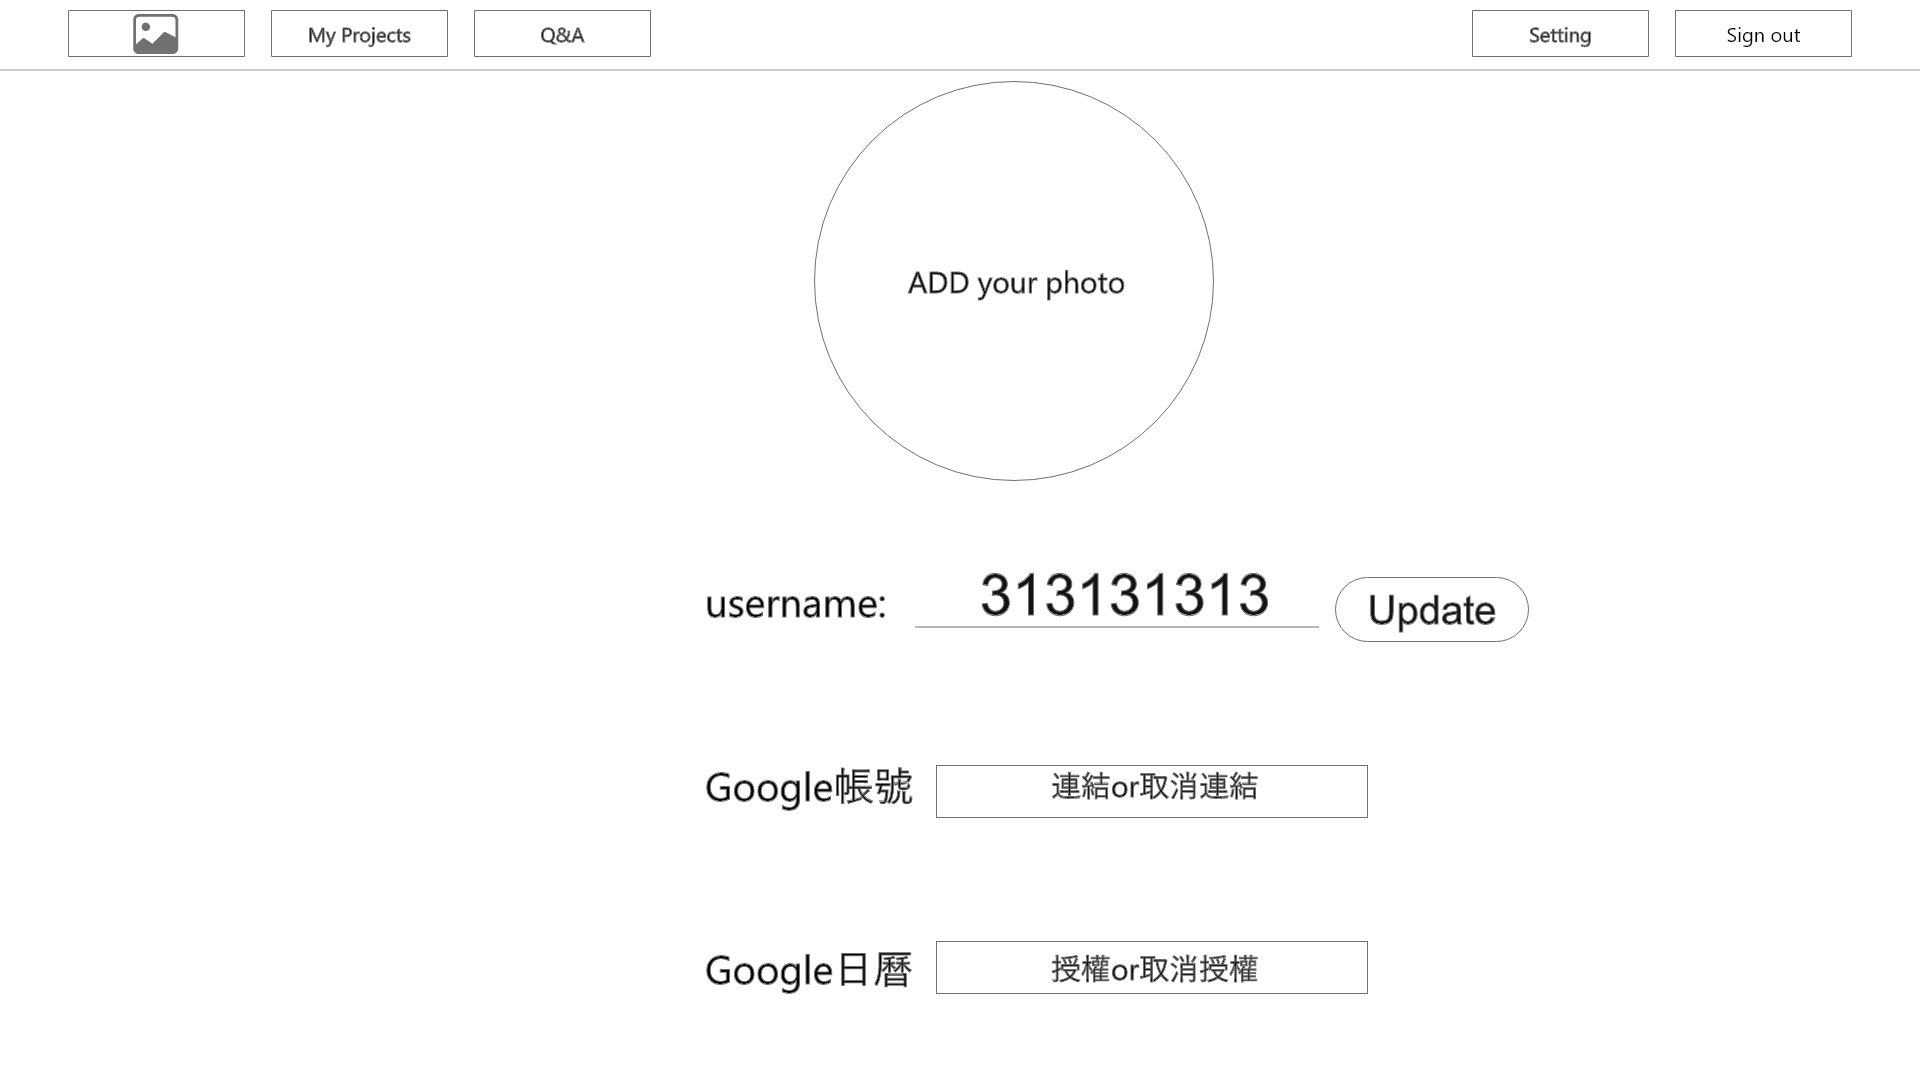
\includegraphics[width=\textwidth]{assets/wireframe/setting.png}
  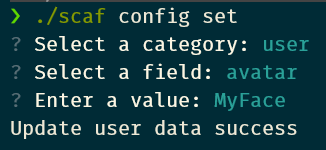
\includegraphics[width=\textwidth]{assets/wireframe/setting_photo_CLI.png}
  \item 更改自己的名稱: 小林因為覺得中二的專案名稱被刪掉了很可惜,所以想要把自己的名稱搞的中二一點來平衡一下。\\
  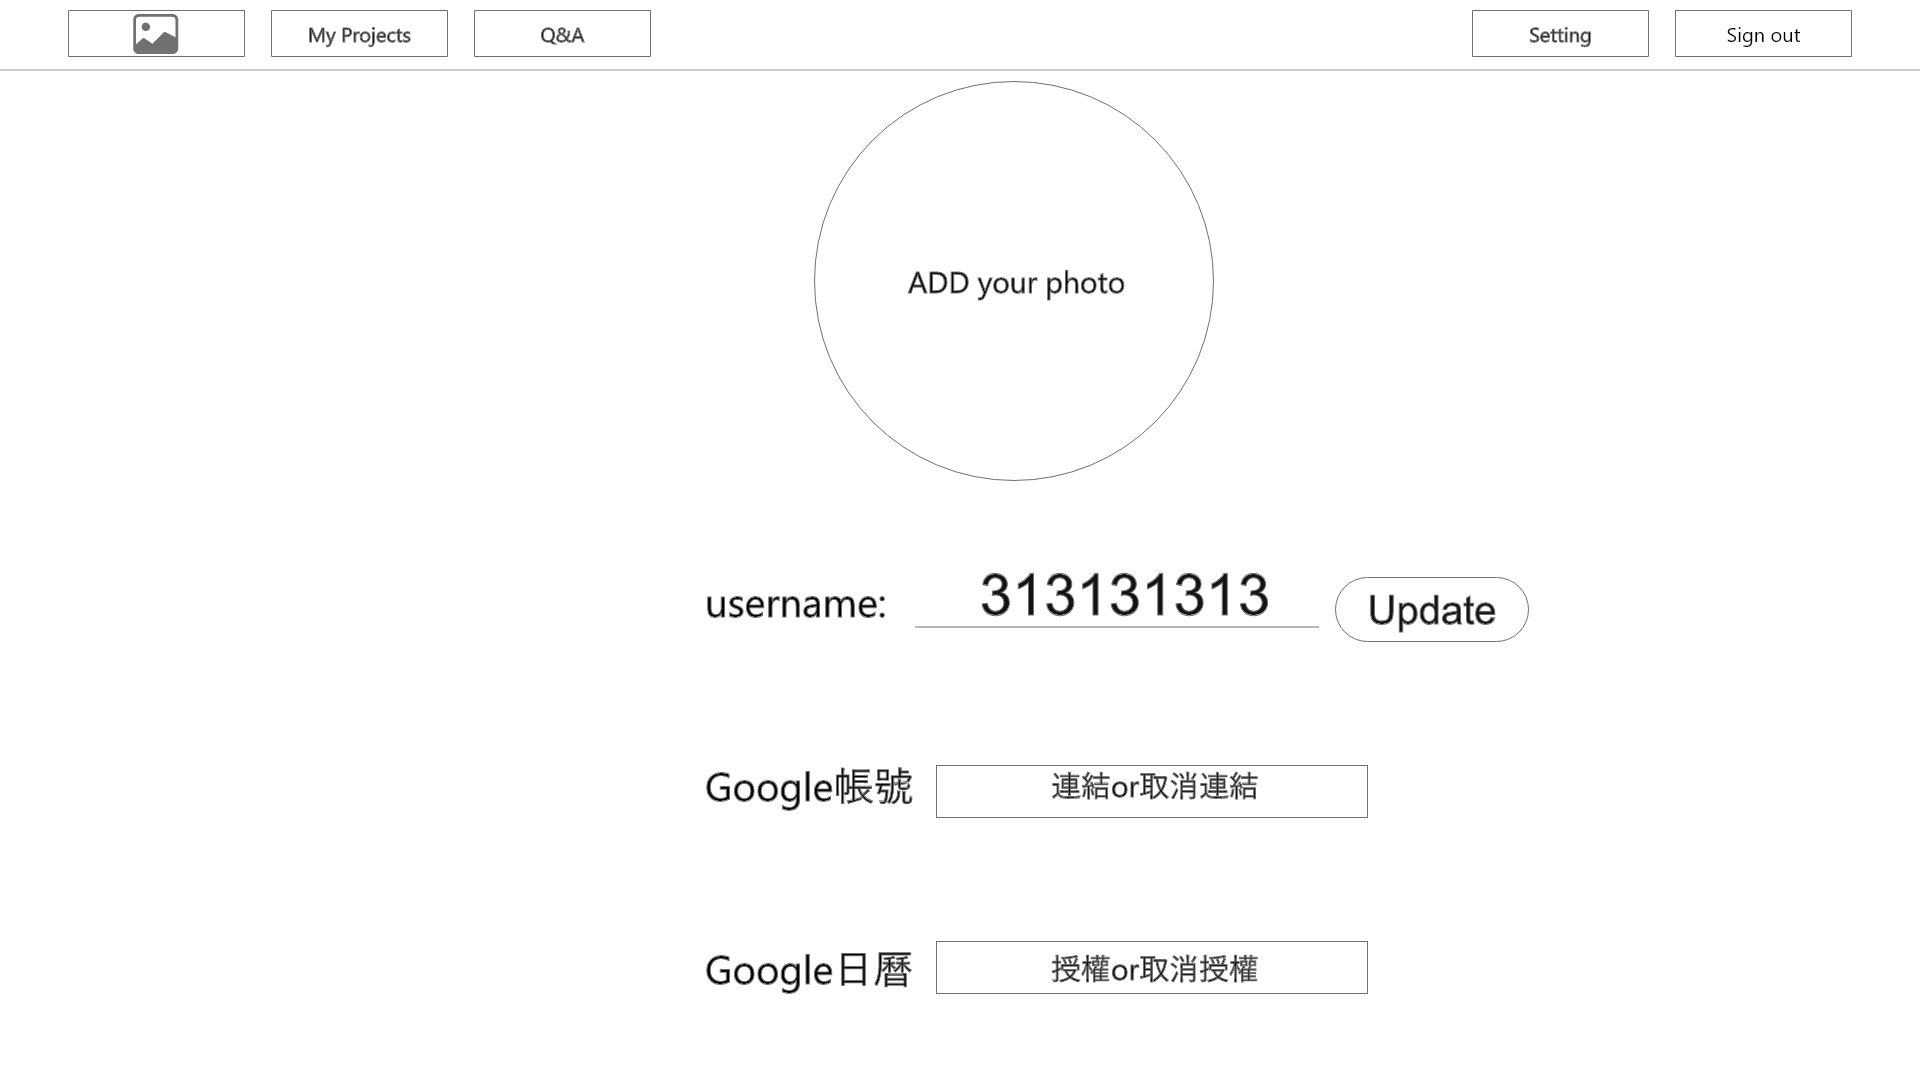
\includegraphics[width=\textwidth]{assets/wireframe/setting.png}
  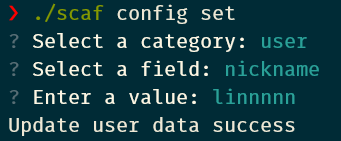
\includegraphics[width=\textwidth]{assets/wireframe/setting_name_CLI.png}
  \item 授權帳號: 小林想利用自己的Google日曆來分配自己開發階段的期限,於是按下授權鍵給Google日曆授權。\\
  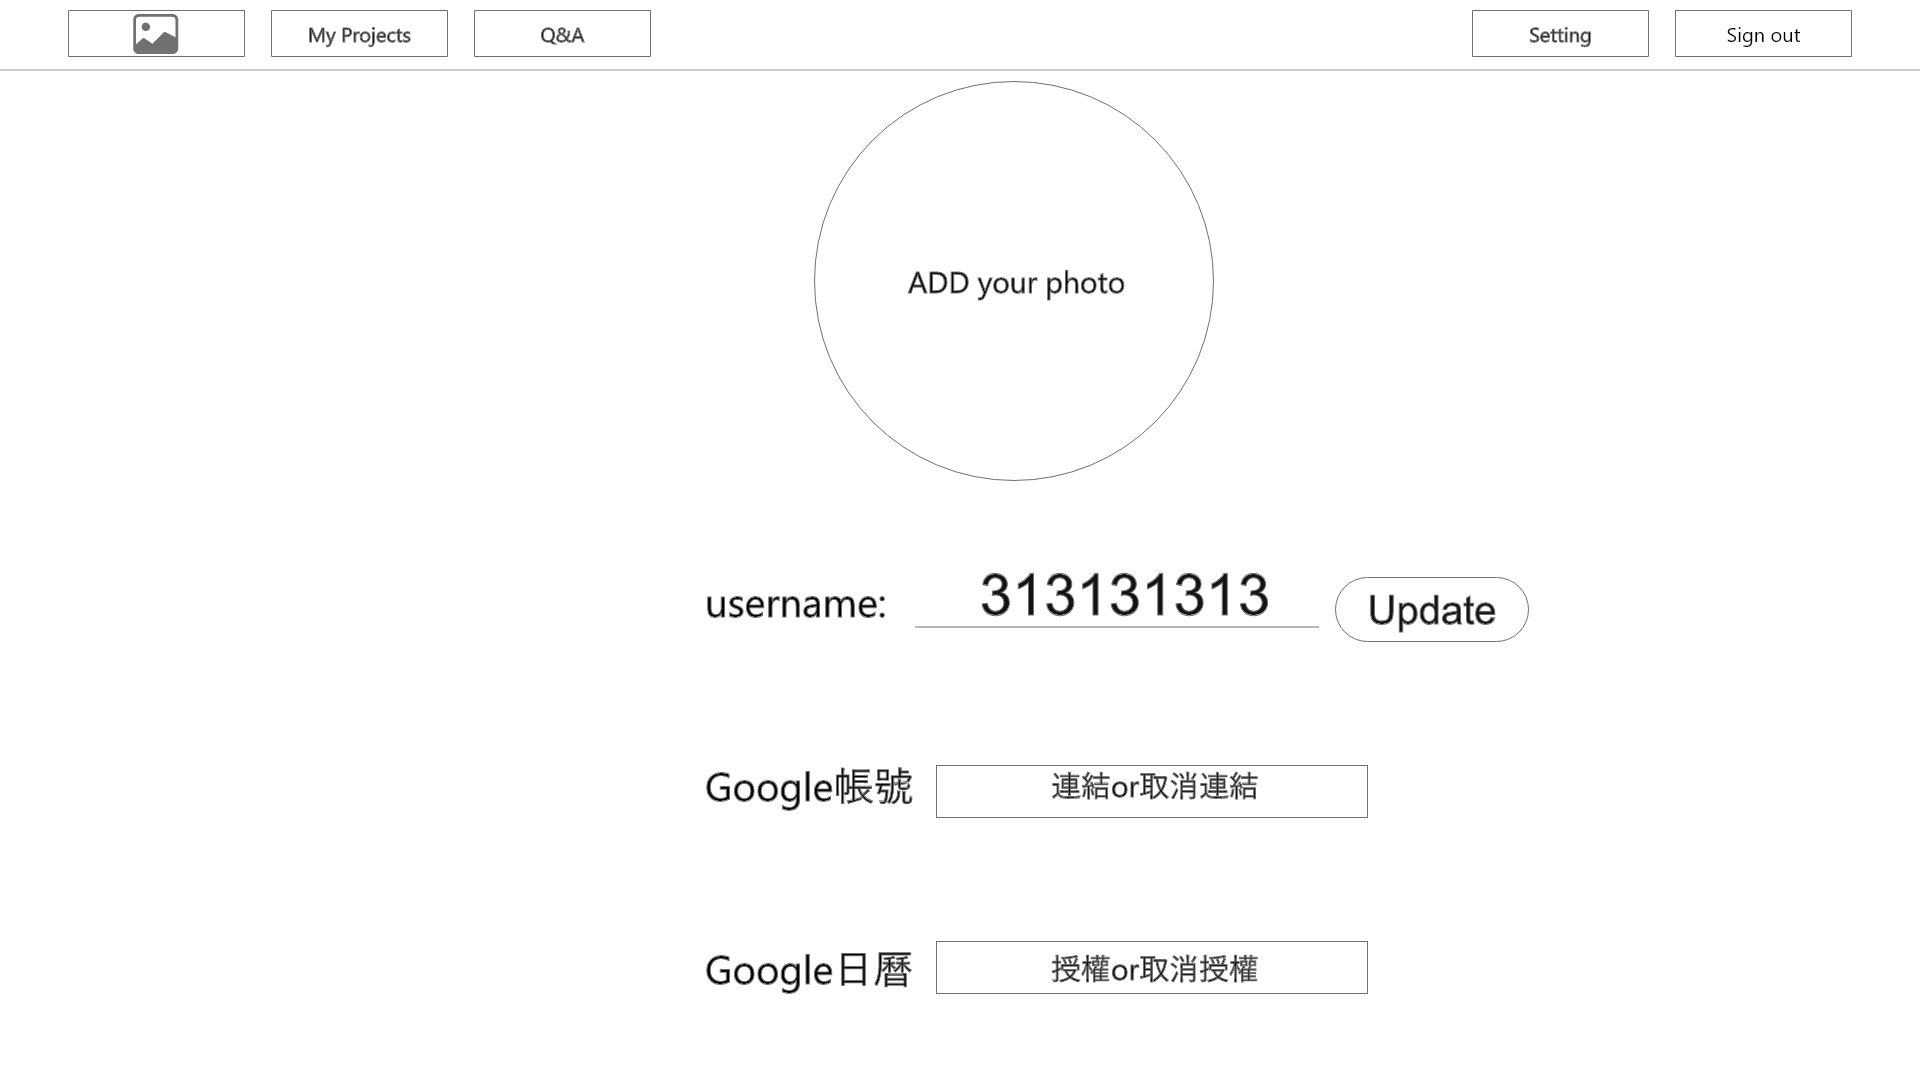
\includegraphics[width=\textwidth]{assets/wireframe/setting.png}
  \item 使用CLI工具: 小林想了解該如何使用CLI工具,所以在終端機使用scaf的指令,就可以進一步了解如何使用子指令。\\
  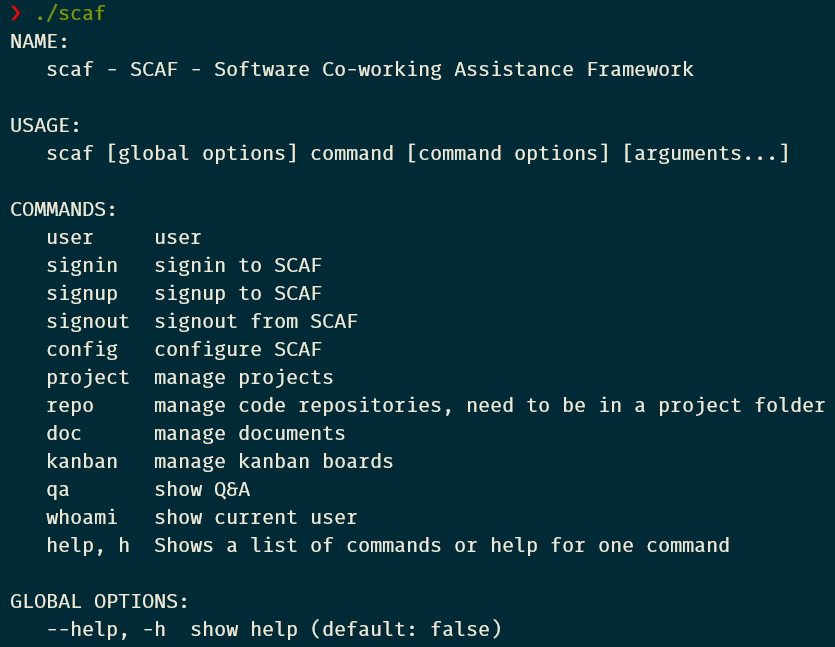
\includegraphics[width=\textwidth]{assets/wireframe/cli.png}
\end{enumerate}

\subsection*{4. 功能需求(Feature Requirements)}               

\begin{tabularx}{\textwidth}{
  |p{\dimexpr.2\linewidth-2\tabcolsep-1.33333\arrayrulewidth}%
  |p{\dimexpr.2\linewidth-2\tabcolsep-1.33333\arrayrulewidth}%
  |p{\dimexpr.6\linewidth-2\tabcolsep-1.33333\arrayrulewidth}|%
}
  \hline
  功能編號 & 功能名稱 & 功能說明 \\ \hline
  SCAF-FR-01 & 登入 & 使用者可以用 email 跟密碼進行登入\\ \hline
  SCAF-FR-02 & 註冊 & 使用者可以用 email 註冊新帳戶。 \\ \hline
  SCAF-FR-03 & 忘記密碼 & 使用者可以發送驗證碼至 email 並重設密碼。 \\ \hline
  SCAF-FR-04 & 共用專案 & 使用者可以分享連結讓多人參與共同編輯。 \\ \hline
  SCAF-FR-05 & 開發流程模式 & 使用者可以選擇自己想要的設計流程。 \\ \hline
  SCAF-FR-06 & 專案初始化 & 使用者可以生成專案並選擇是否加入README。 \\ \hline
  SCAF-FR-07 & 可以加入任意連結作為 repository 連結 & 使用者在同一個專案中可以共同使用reository(Github)。 \\ \hline
  SCAF-FR-08 & 輸入文件 (需求、設計等) & 使用者編輯相關文件。 \\ \hline
  SCAF-FR-09 & 工作計畫排程 & 使用者可以利用看板、行事曆,來查看專案的排程。 \\ \hline
  SCAF-FR-10 & 通知 & 使用者接收專案內的更動通知、其他專案的邀請。 \\ \hline
  SCAF-FR-11 & 設定 & 使用者可以更改自己的名稱、信箱、自介、密碼。 \\ \hline
  SCAF-FR-12 & 問答 & 使用者可以在Q\&A文件中查詢自己的問題,並尋找答案。 \\ \hline
  SCAF-FR-13 & Google 日曆授權 & 使用者可以授權給Google日曆來安排行程。 \\ \hline 
  SCAF-FR-14 & 專案設定修改 & 使用者(專案擁有者)可以對專案進行名稱、人員變更。 \\ \hline
\end{tabularx}

\subsection*{5. 非功能需求(Non-functional Requirements)}

\begin{tabularx}{\textwidth}{
  |p{\dimexpr.3\linewidth-2\tabcolsep-2\arrayrulewidth}%
  |p{\dimexpr.7\linewidth-2\tabcolsep-2\arrayrulewidth}|%
}
  \hline
  功能編號 &  功能說明 \\ \hline
  SCAF-NFP-01 & 系統人數同時負荷 1000 人 \\ \hline
  SCAF-NFP-02 & 回應時間在 1 秒內 \\ \hline
  SCAF-NFP-03 & 使用 Https 加密傳輸 \\ \hline
  SCAF-NFP-04 & CSRF 防護 \\ \hline
  SCAF-NFP-05 & 防止 DDoS 攻擊 \\ \hline
  SCAF-NFP-06 & Q\&A 搜尋結果在 1 秒內回應 \\ \hline
\end{tabularx}

\end{document}